%%%%%%%%%%%%%%%%%%%%%%%%%%%%%%%%%%%%%%%%%
% Beamer Presentation
% LaTeX Template
% Version 1.0 (10/11/12)
%
% This template has been downloaded from:
% http://www.LaTeXTemplates.com
%
% License:
% CC BY-NC-SA 3.0 (http://creativecommons.org/licenses/by-nc-sa/3.0/)
%
%%%%%%%%%%%%%%%%%%%%%%%%%%%%%%%%%%%%%%%%%

%----------------------------------------------------------------------------------------
%	PACKAGES AND THEMES
%----------------------------------------------------------------------------------------

\documentclass{beamer}

\mode<presentation> {

% The Beamer class comes with a number of default slide themes
% which change the colors and layouts of slides. Below this is a list
% of all the themes, uncomment each in turn to see what they look like.

%\usetheme{default}
%\usetheme{AnnArbor}
%\usetheme{Antibes}
%\usetheme{Bergen}
%\usetheme{Berkeley}
%\usetheme{Berlin}
\usetheme{Boadilla}
%\usetheme{CambridgeUS}
%\usetheme{Copenhagen}
%\usetheme{Darmstadt}
%\usetheme{Dresden}
%\usetheme{Frankfurt}
%\usetheme{Goettingen}
%\usetheme{Hannover}
%\usetheme{Ilmenau}
%\usetheme{JuanLesPins}
%\usetheme{Luebeck}
% \usetheme{Madrid}
%\usetheme{Malmoe}
%\usetheme{Marburg}
%\usetheme{Montpellier}
%\usetheme{PaloAlto}
%\usetheme{Pittsburgh}
%\usetheme{Rochester}
%\usetheme{Singapore}
%\usetheme{Szeged}
%\usetheme{Warsaw}

% As well as themes, the Beamer class has a number of color themes
% for any slide theme. Uncomment each of these in turn to see how it
% changes the colors of your current slide theme.

%\usecolortheme{albatross}
%\usecolortheme{beaver}
%\usecolortheme{beetle}
%\usecolortheme{crane}
%\usecolortheme{dolphin}
%\usecolortheme{dove}
%\usecolortheme{fly}
%\usecolortheme{lily}
%\usecolortheme{orchid}
%\usecolortheme{rose}
%\usecolortheme{seagull}
%\usecolortheme{seahorse}
%\usecolortheme{whale}
%\usecolortheme{wolverine}

%\setbeamertemplate{footline} % To remove the footer line in all slides uncomment this line
%\setbeamertemplate{footline}[page number] % To replace the footer line in all slides with a simple slide count uncomment this line

\setbeamertemplate{navigation symbols}{} % To remove the navigation symbols from the bottom of all slides uncomment this line
}

\usepackage{graphicx} % Allows including images
\graphicspath{ {../img/} }
\usepackage{booktabs} % Allows the use of \toprule, \midrule and \bottomrule in tables
\usepackage{subcaption} % Allows using subfigures
\captionsetup{compatibility=false}
\usepackage{multirow}
\usepackage{rotating}
\usepackage{pifont}
%
\fboxsep=0pt
\fboxrule=2pt
%


%----------------------------------------------------------------------------------------
%	TITLE PAGE
%----------------------------------------------------------------------------------------

\title[Interface of 3D Reconstruction]{Development and Application of a Description-based Interface for 3D Object Reconstruction} % The short title appears at the bottom of every slide, the full title is only on the title page

\author{Kai Wu} % Your name
\institute[UBC] % Your institution as it will appear on the bottom of every slide, may be shorthand to save space
{
University of British Columbia \\ % Your institution for the title page
\medskip
\textit{kaywu@ece.ubc.ca} \\ % Your email address
% \textit{Website: }\href{https://imkaywu.github.io/3drecon_dataset/}{3DRecon Dataset}
}
\date{\today} % Date, can be changed to a custom date

\begin{document}

\begin{frame}
\titlepage % Print the title page as the first slide
\end{frame}

\begin{frame}
\frametitle{Table of Contents} % Table of contents slide, comment this block out to remove it
\tableofcontents % Throughout your presentation, if you choose to use \section{} and \subsection{} commands, these will automatically be printed on this slide as an overview of your presentation
\end{frame}

%----------------------------------------------------------------------------------------
%	PRESENTATION SLIDES
%----------------------------------------------------------------------------------------
%------------------------------------------------
\section{Motivation}
%------------------------------------------------
\begin{frame}
\tableofcontents[currentsection,currentsubsection, 
    hideothersubsections, 
    sectionstyle=show/shaded,]
\end{frame}

%------------------------------------------------
\begin{frame}
\frametitle{Motivation: traditional 3D Reconstruction}

\begin{figure}
\centering
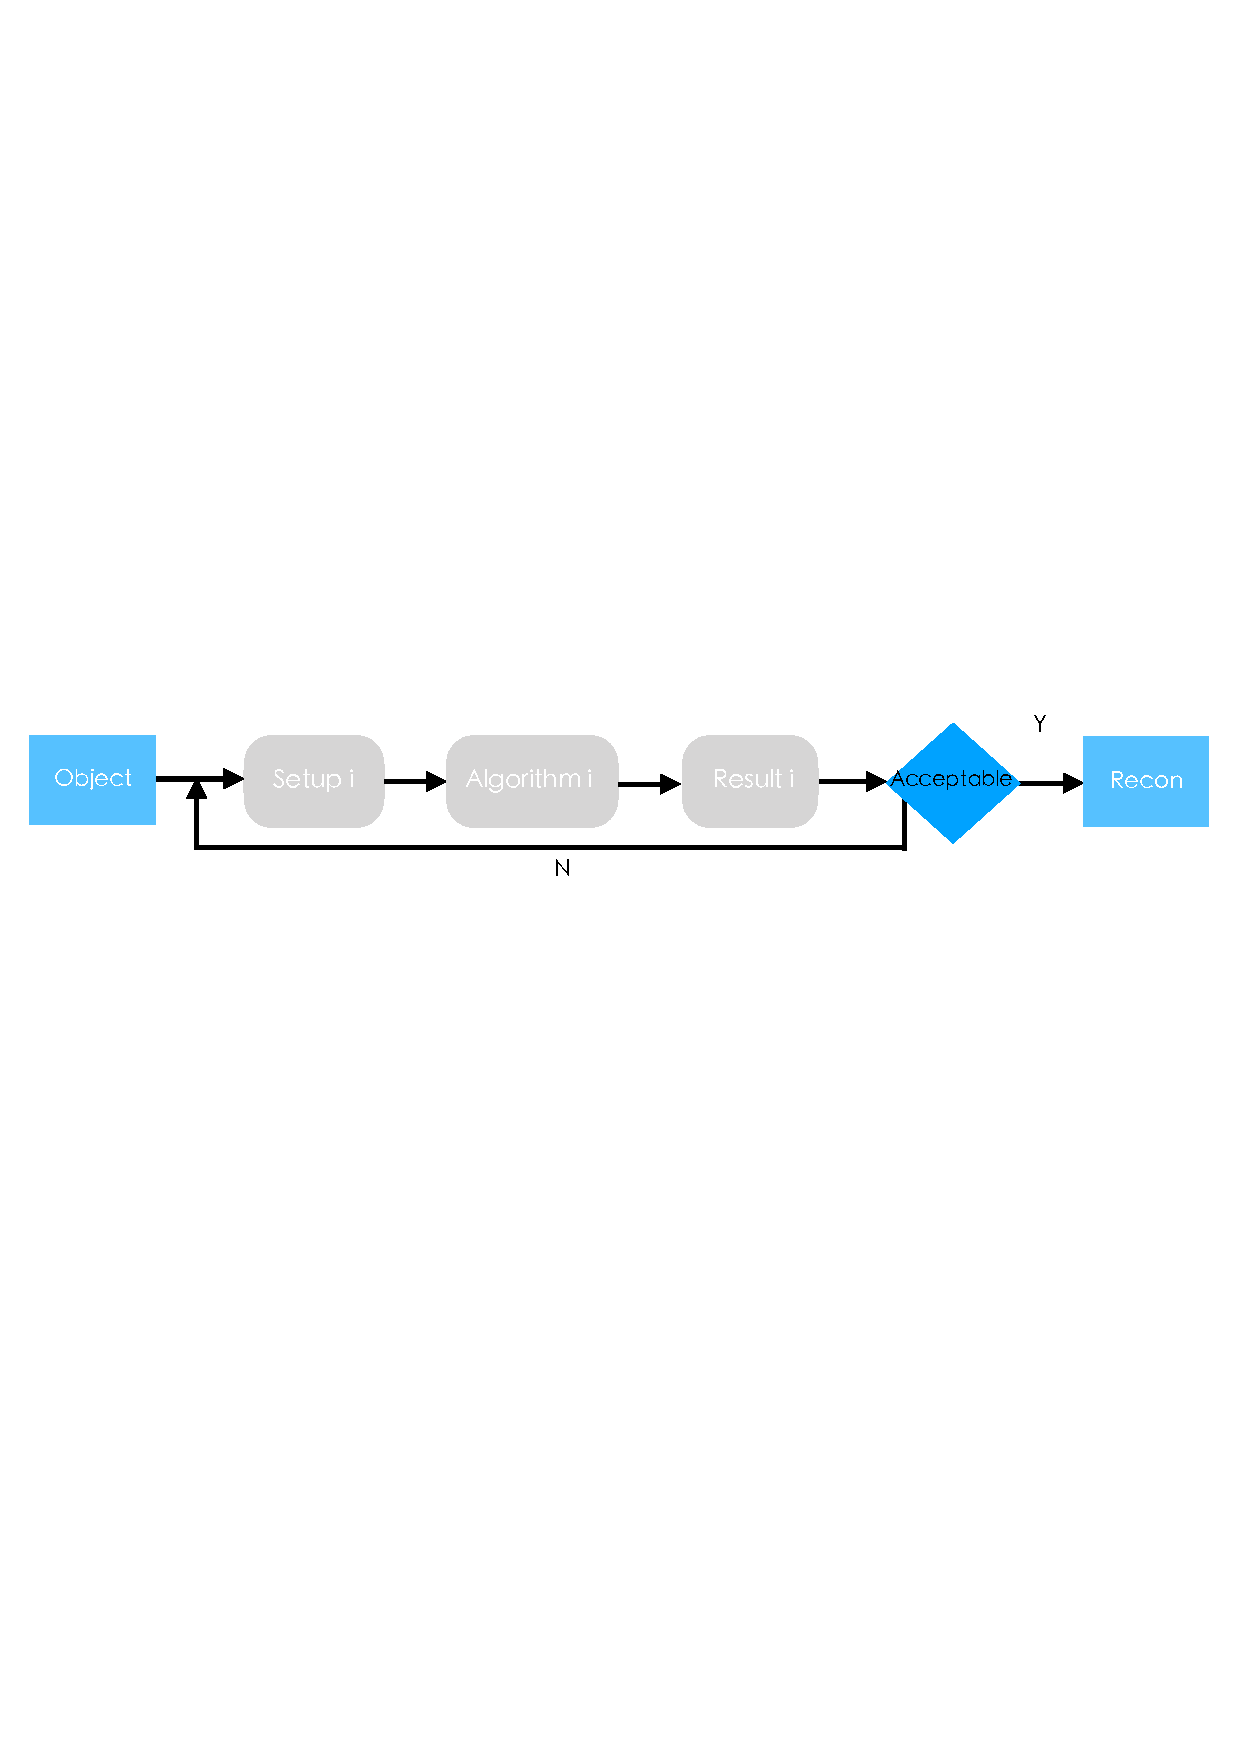
\includegraphics[width=0.8\textwidth]{images/traditional_3d_vision.pdf}
\end{figure}

\begin{itemize}
\item Hardware setup: calibration, controlled environment
\item Algorithms: vision background
\item Results: keep trying until an acceptable result
\end{itemize}

\end{frame}


%------------------------------------------------
\begin{frame}
\frametitle{Motivation: interface to 3D Reconstruction}
What if we can create an interface above the 3D algorithms, which can select an appropriate algorithm based on users' description, and achieve a successful reconstruction result.

\begin{figure}
\centering
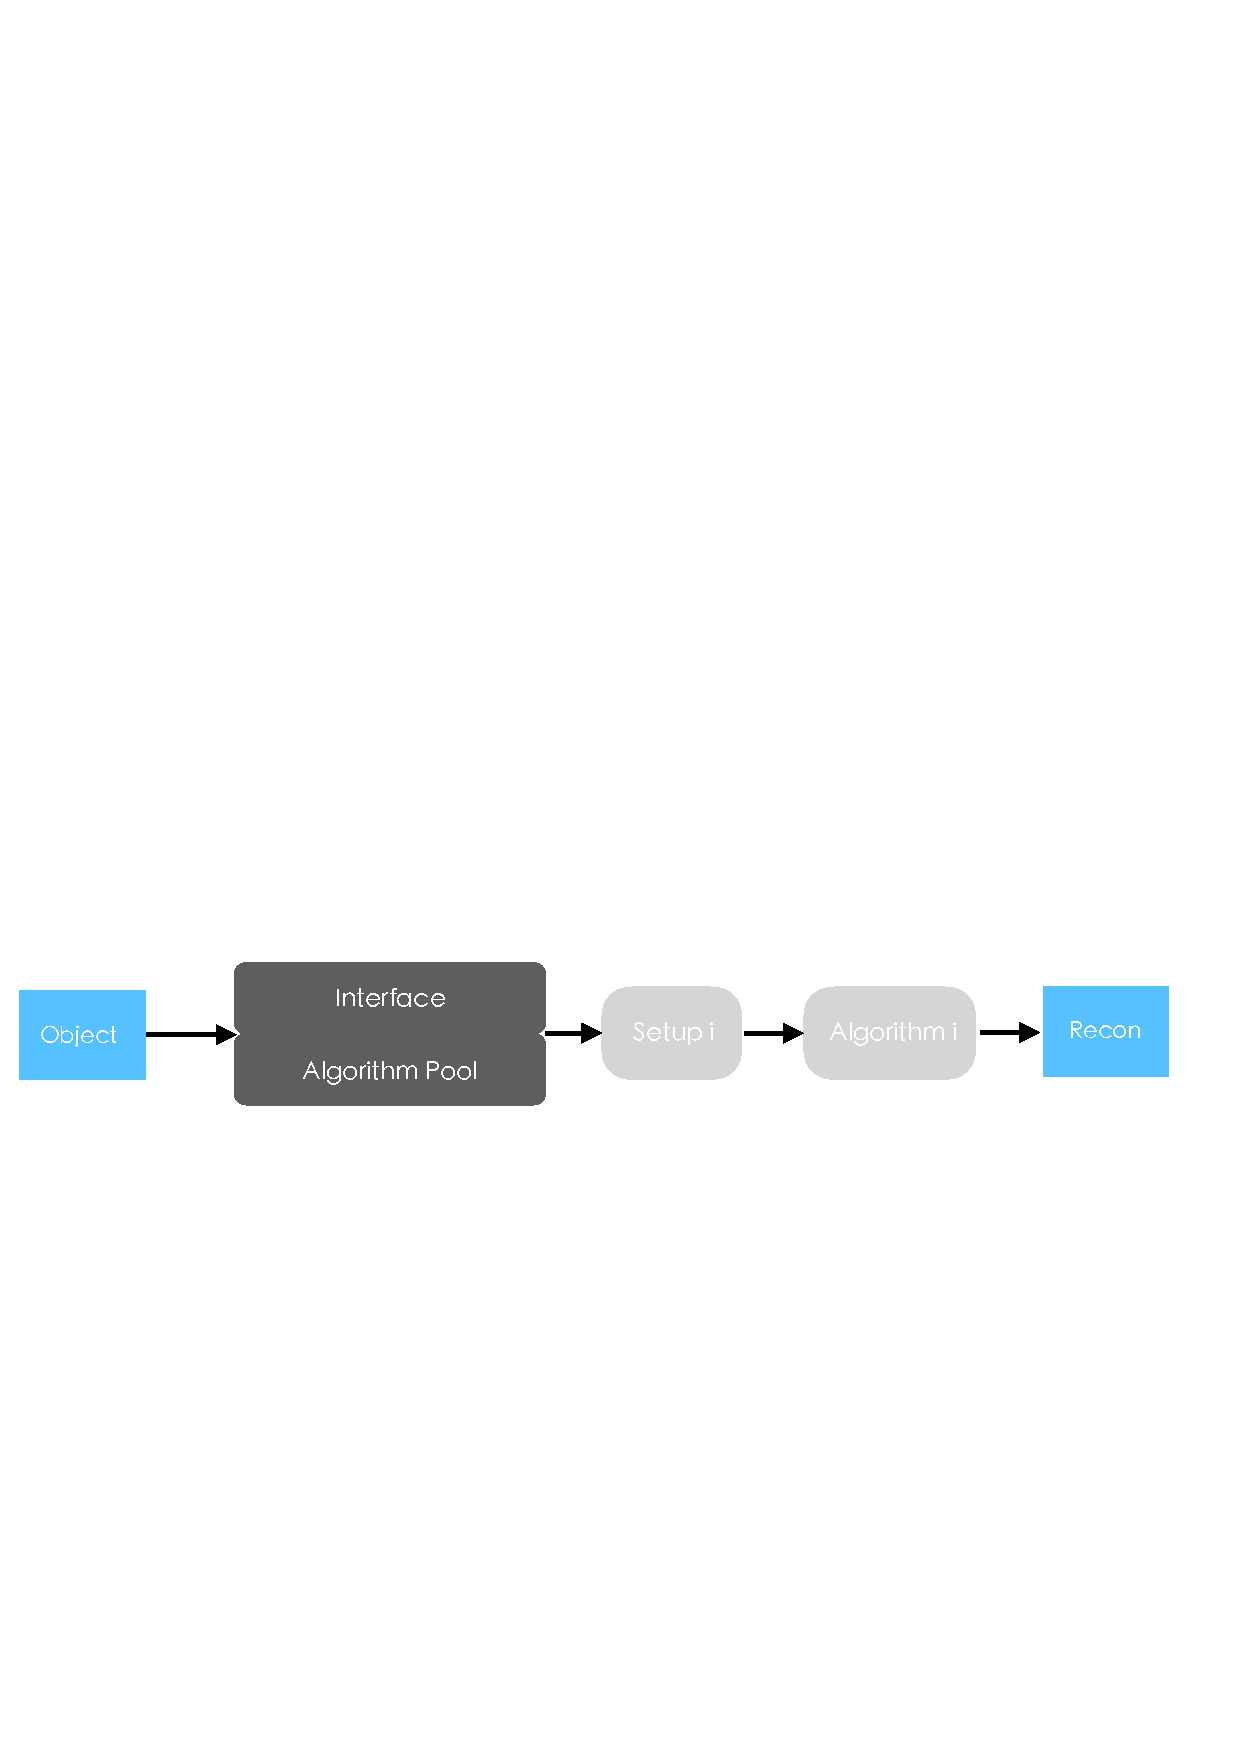
\includegraphics[width=0.8\textwidth]{images/interface_3d_vision.pdf}
\end{figure}

\end{frame}

%------------------------------------------------
\section{Contribution}
%------------------------------------------------

\begin{frame}
\tableofcontents[currentsection,currentsubsection, 
    hideothersubsections, 
    sectionstyle=show/shaded,]
\end{frame}

%------------------------------------------------
\begin{frame}
\frametitle{Contribution}
Development of an interface for 3D reconstruction problem, which hides algorithmic details and allows users to describe conditions surrounding the problem. This description can be interpreteded so that an appropriate algorithm is chosen to obtain a successful reconstruction result.
\end{frame}

%------------------------------------------------
\begin{frame}
\frametitle{Contribution (cont'd)}
This contribution is significant because:
\begin{itemize}
\item No single algorithm can work for a diverse categories of objects. The interface, to some extent, can cover a wider range of object categories by incorporating multiple algorithms.
\item An description is provides that hides the algorithmic details, thus understanding of the algorithm, or conditions to apply a specific algorithm is not a prerequisite.
\end{itemize}
\end{frame}

%------------------------------------------------
% \section{Overview}
%------------------------------------------------

% \begin{frame}
% \frametitle{Overview}
% \tableofcontents[currentsection,currentsubsection, 
%     hideothersubsections, 
%     sectionstyle=show/shaded,]
% \end{frame}

%------------------------------------------------

% \begin{frame}
% \frametitle{Overview}

% \begin{itemize}
% \item \textbf{Taxonomy}: change the way of viewing algorithms, not from an algorithmic viewpoint, but from a problem-oriented (object-centered) viewpoint.
% \item \textbf{Description}: how to describe a sub-space in the $n-$dimensional problem space so that the conditions that an algorithm works reliably can be well defined;
% \item \textbf{Mapping}: discover the mapping between algorithms and the sub-spaces in the $n-$dimensional problem space.
% \item \textbf{Interpretation}: test the interpretability of the interface using synthetic and real-world datasets.
% \end{itemize}
% \end{frame}

%------------------------------------------------
\section{Related Work}
%------------------------------------------------

\begin{frame}
\tableofcontents[currentsection,currentsubsection, 
    hideothersubsections, 
    sectionstyle=show/shaded,]
\end{frame}

%------------------------------------------------
\begin{frame}
\frametitle{Related Work}

Previous algorithm taxonomy based on visual/geometric cues.
\begin{figure}
\begin{tabular}{cccc}
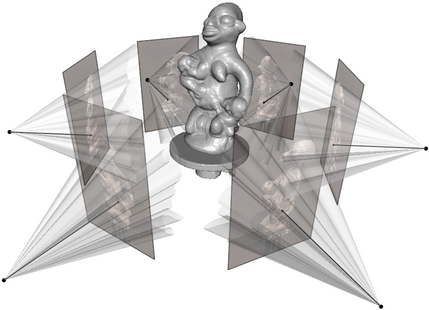
\includegraphics[width=0.25\textwidth]{images/mvs.png} &
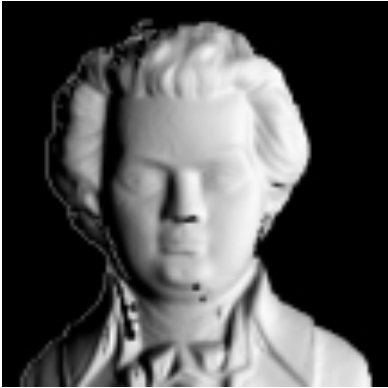
\includegraphics[width=0.2\textwidth]{images/sfs.png} & 
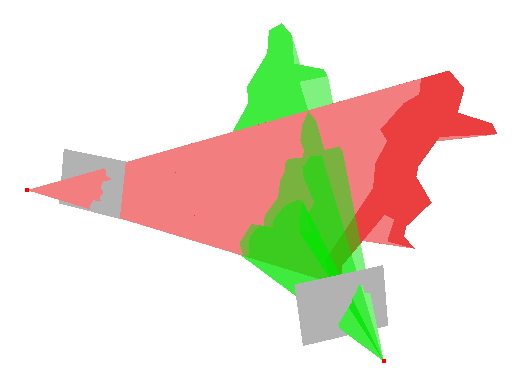
\includegraphics[width=0.25\textwidth]{images/vh.jpg}\\
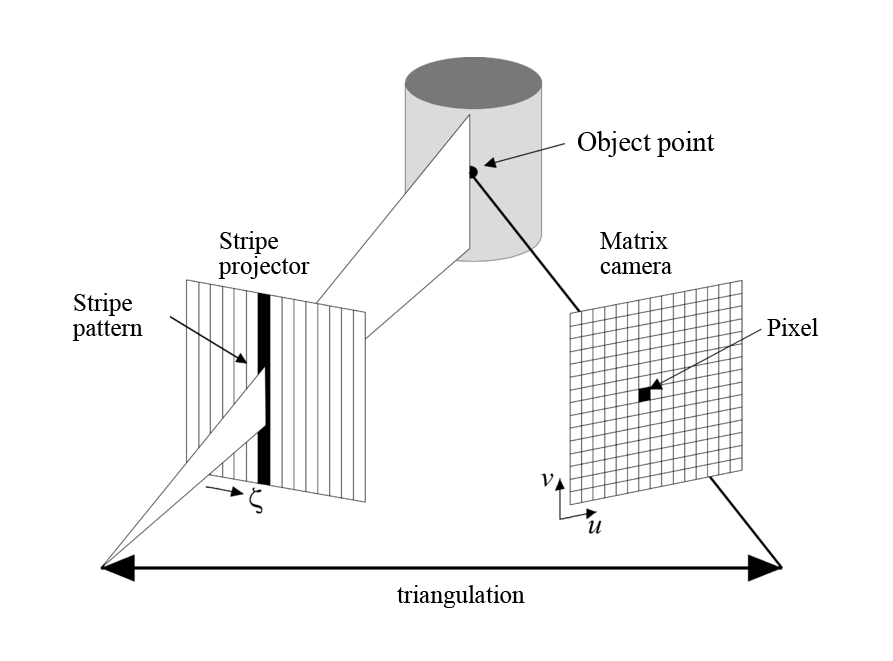
\includegraphics[width=0.25\textwidth]{images/sl.jpg} & 
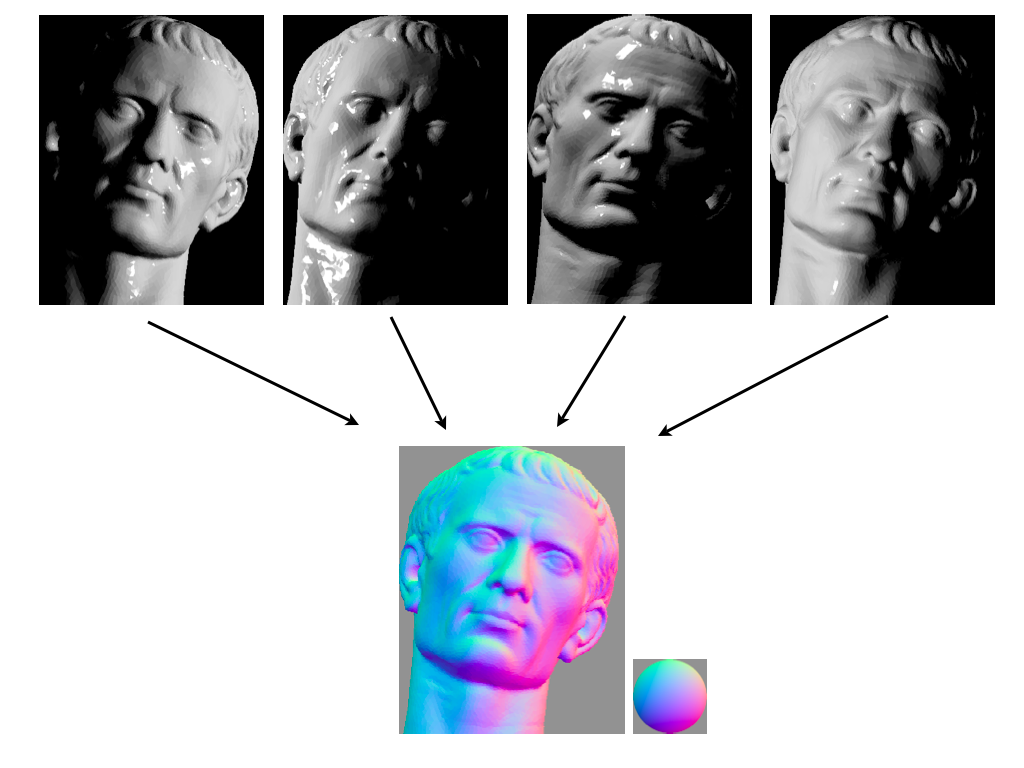
\includegraphics[width=0.25\textwidth]{images/ps.png} &
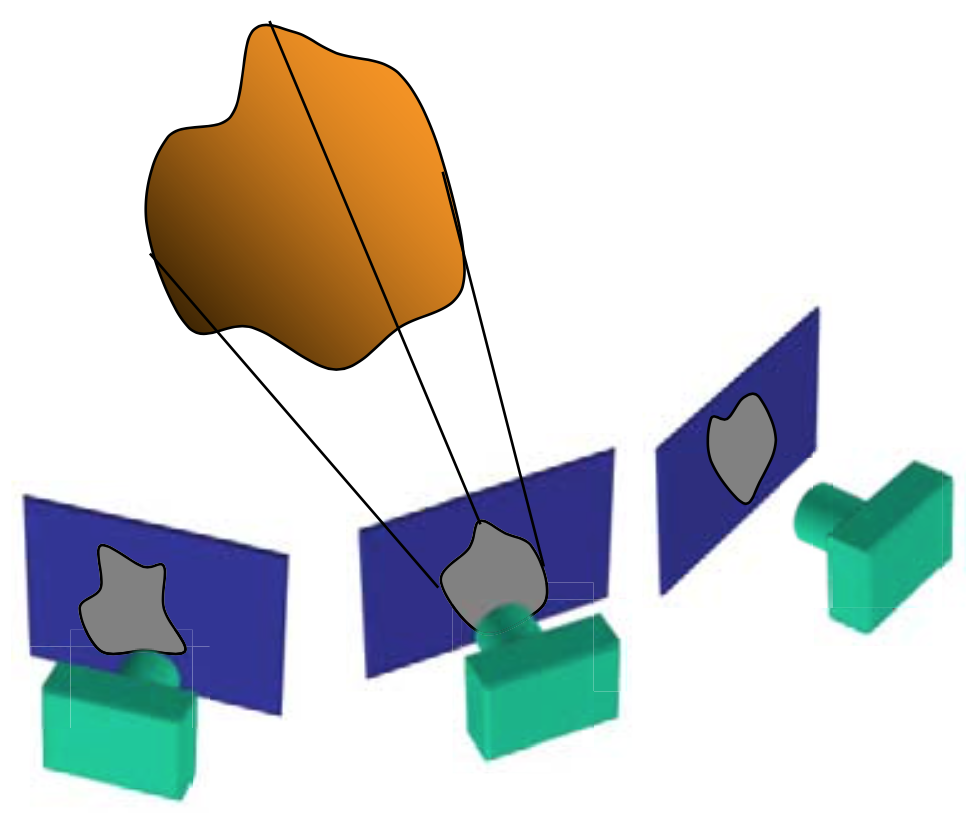
\includegraphics[width=0.25\textwidth]{images/vh_1.png}\\
(a). Stereo & (b). Shading & (c) Silhouette \\
\end{tabular}
\end{figure}

\end{frame}

%------------------------------------------------
\section{Development of Interface}
%------------------------------------------------
\begin{frame}
\tableofcontents[currentsection,currentsubsection, 
    hideothersubsections, 
    sectionstyle=show/shaded,]
\end{frame}

%------------------------------------------------
\subsection{Problem Space of 3D Reconstruction}
%------------------------------------------------
\begin{frame}
\frametitle{Taxonomy: properties of problem space}

\begin{itemize}
\item \textit{algorithm-centered} taxonomy categorizes algorithms based on algorithmic details, as discussed in \textbf{Related Work};
\item \textit{object-centered} taxonomy categorizes algorithms based on the problem conditions that the algorithm can reliably works under.
\end{itemize}

\begin{figure}[h]
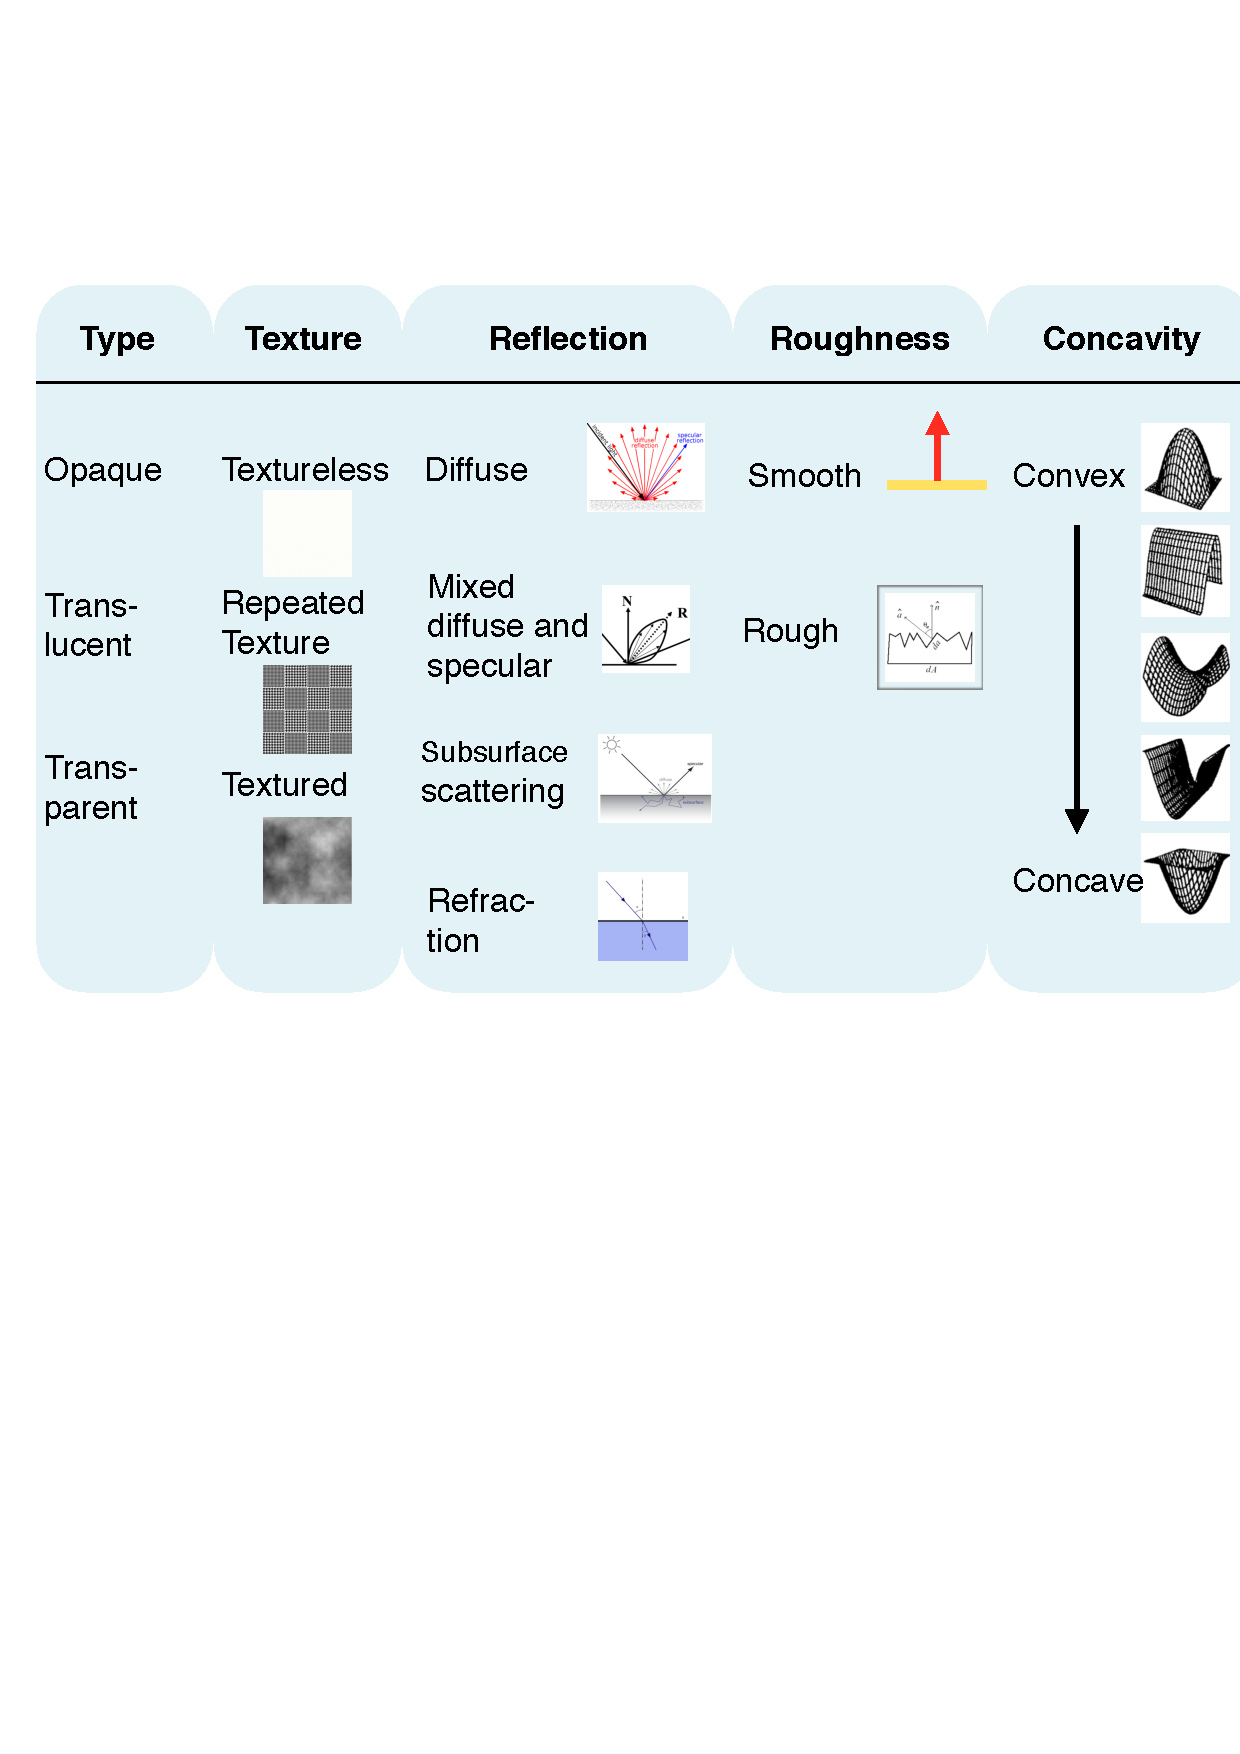
\includegraphics[width=0.7\textwidth]{taxo/obj_class}
\end{figure}

\end{frame}

%------------------------------------------------
\begin{frame}
\frametitle{Taxonomy: six problem conditions}

\begin{figure}[h]
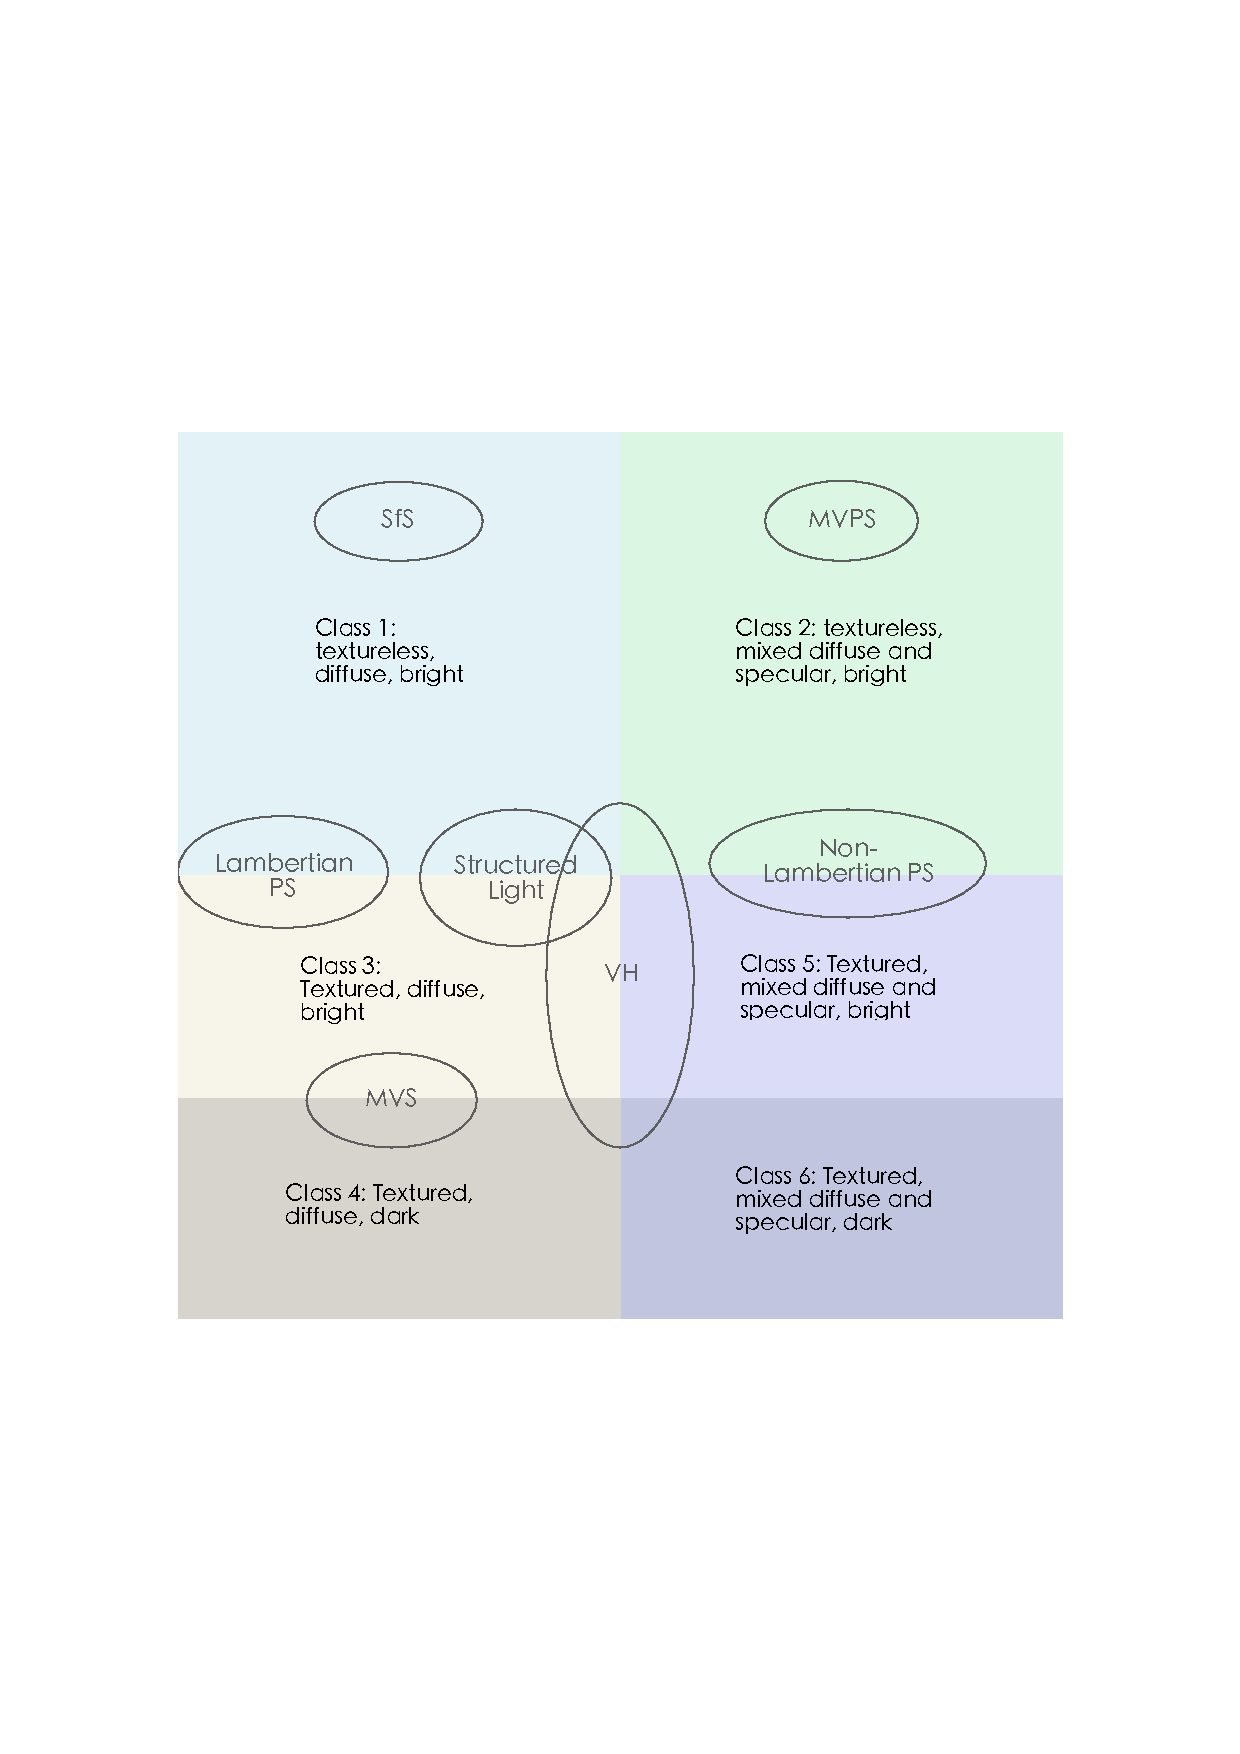
\includegraphics[width=0.6\textwidth]{taxo/six_class}
\end{figure}

\end{frame}

%------------------------------------------------
\subsection{Description of 3D Reconstruction}
%------------------------------------------------
\begin{frame}
\frametitle{Description: model and representations}

\begin{table}[!htbp]
  \centering
  \begin{tabular}{l|ll}
  \toprule
  \textbf{Model} & \textbf{Representation} & \textbf{Visualization}\\
  \midrule
  Texture & \textit{Texture randomness} & \raisebox{-.3\height}{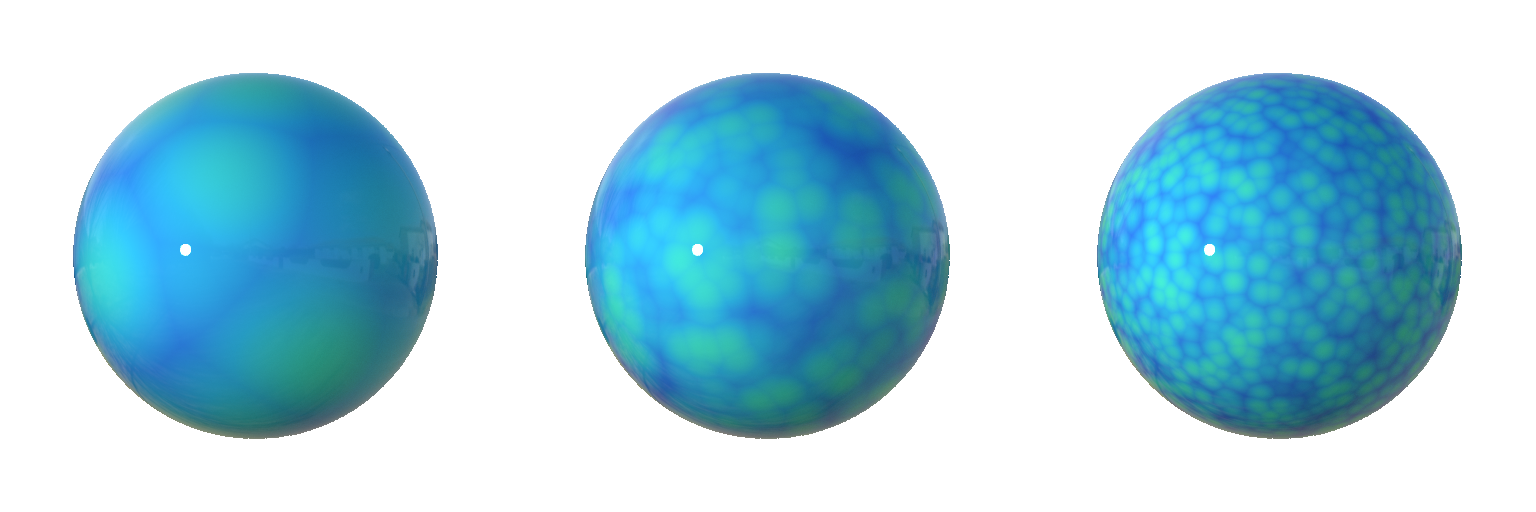
\includegraphics[width=0.4\textwidth]{images/tex.png}}\\
  Lightness & \textit{Albedo} & \raisebox{-.3\height}{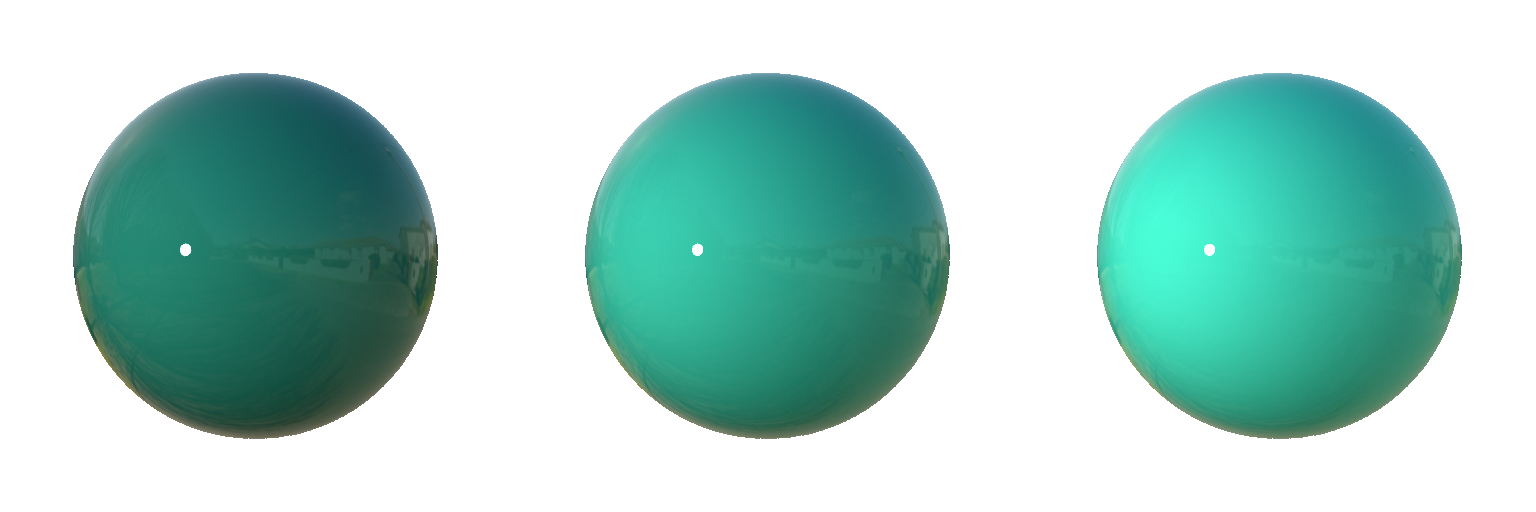
\includegraphics[width=0.4\textwidth]{images/alb.png}}\\
  Specularity & \textit{Specular/diffuse ratio} & \raisebox{-.3\height}{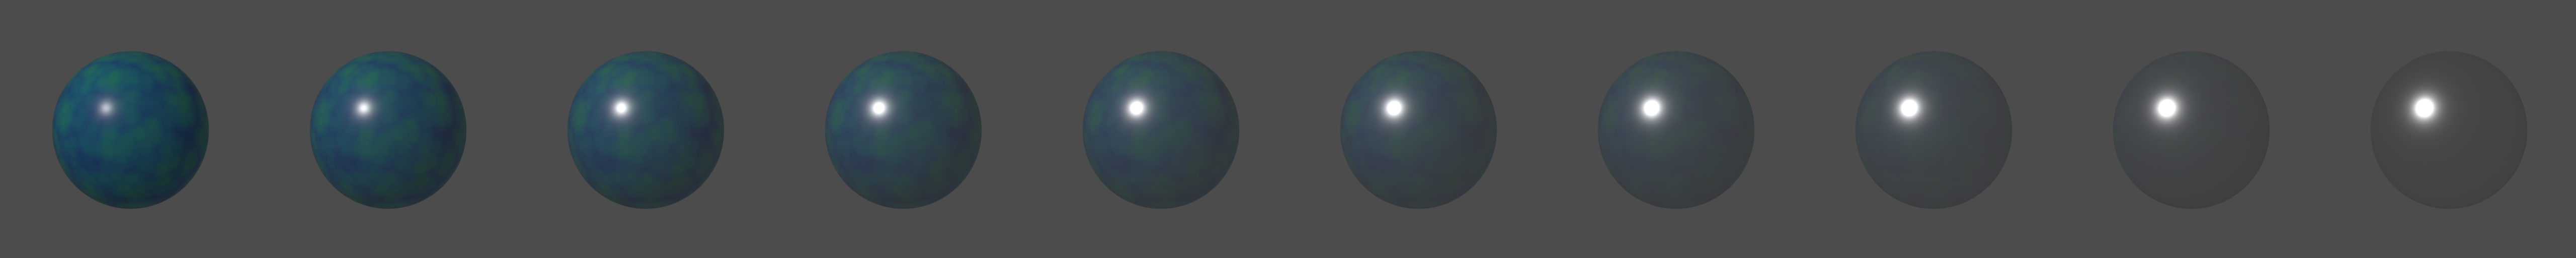
\includegraphics[width=0.4\textwidth]{images/spec.png}}\\
  Roughness & \textit{SD of facet slopes} & \raisebox{-.3\height}{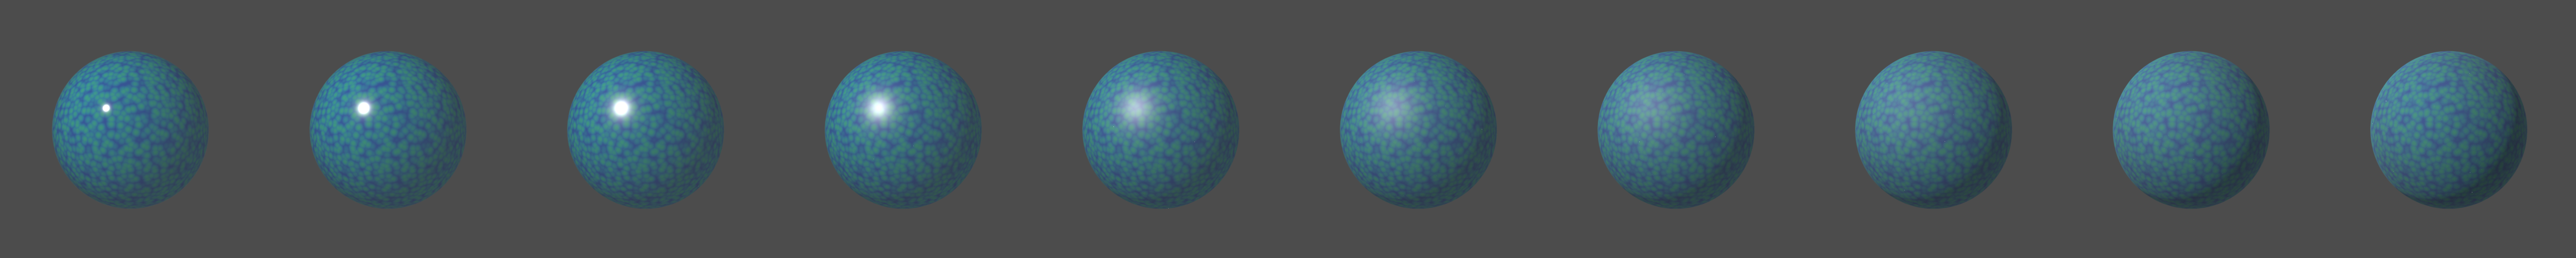
\includegraphics[width=0.4\textwidth]{images/rough.png}}\\
  \bottomrule
  \end{tabular}
  \caption{Representations of the 3D reconstruction problem.}
\end{table}

\end{frame}

%------------------------------------------------
\begin{frame}
\frametitle{Description: expression}

We use three discrete scales to parameterize these properties: \textit{low} (0.2), \textit{medium} (0.5), and \textit{high} (0.8).
\begin{table}[!htbp]
  \centering
  \begin{tabular}{l*{4}{p{1cm}}l}
  \toprule
  \textbf{Object} & Texture & Albedo & Specular & Rough & \textbf{Label}\\
  \midrule
  Class 1 & low/med & high & low/med & high & Tl-B-D-R\\
  Class 2 & low/med & high & high & low/med & Tl-B-M-S\\
  Class 3 & high & high & low/med & high & T-B-D-R\\
  Class 4 & high & high & high & low/med & T-B-M-S\\
  Class 5 & high & low/med & low/med & high & T-D-D-R\\
  Class 6 & high & low/med & high & low/med & T-D-M-S\\
  \bottomrule
  \end{tabular}
  \caption{Expression of the reconstruction problem for the object classss.}
  \label{tab:express}
\end{table}

\end{frame}

%------------------------------------------------
\subsection{Mapping of 3D Reconstruction}
%------------------------------------------------
\begin{frame}
\frametitle{Mapping}

Investigate the problem conditions under which the algorithms can reliably work. This strucure of this chapter is as follows

\begin{figure}
\centering
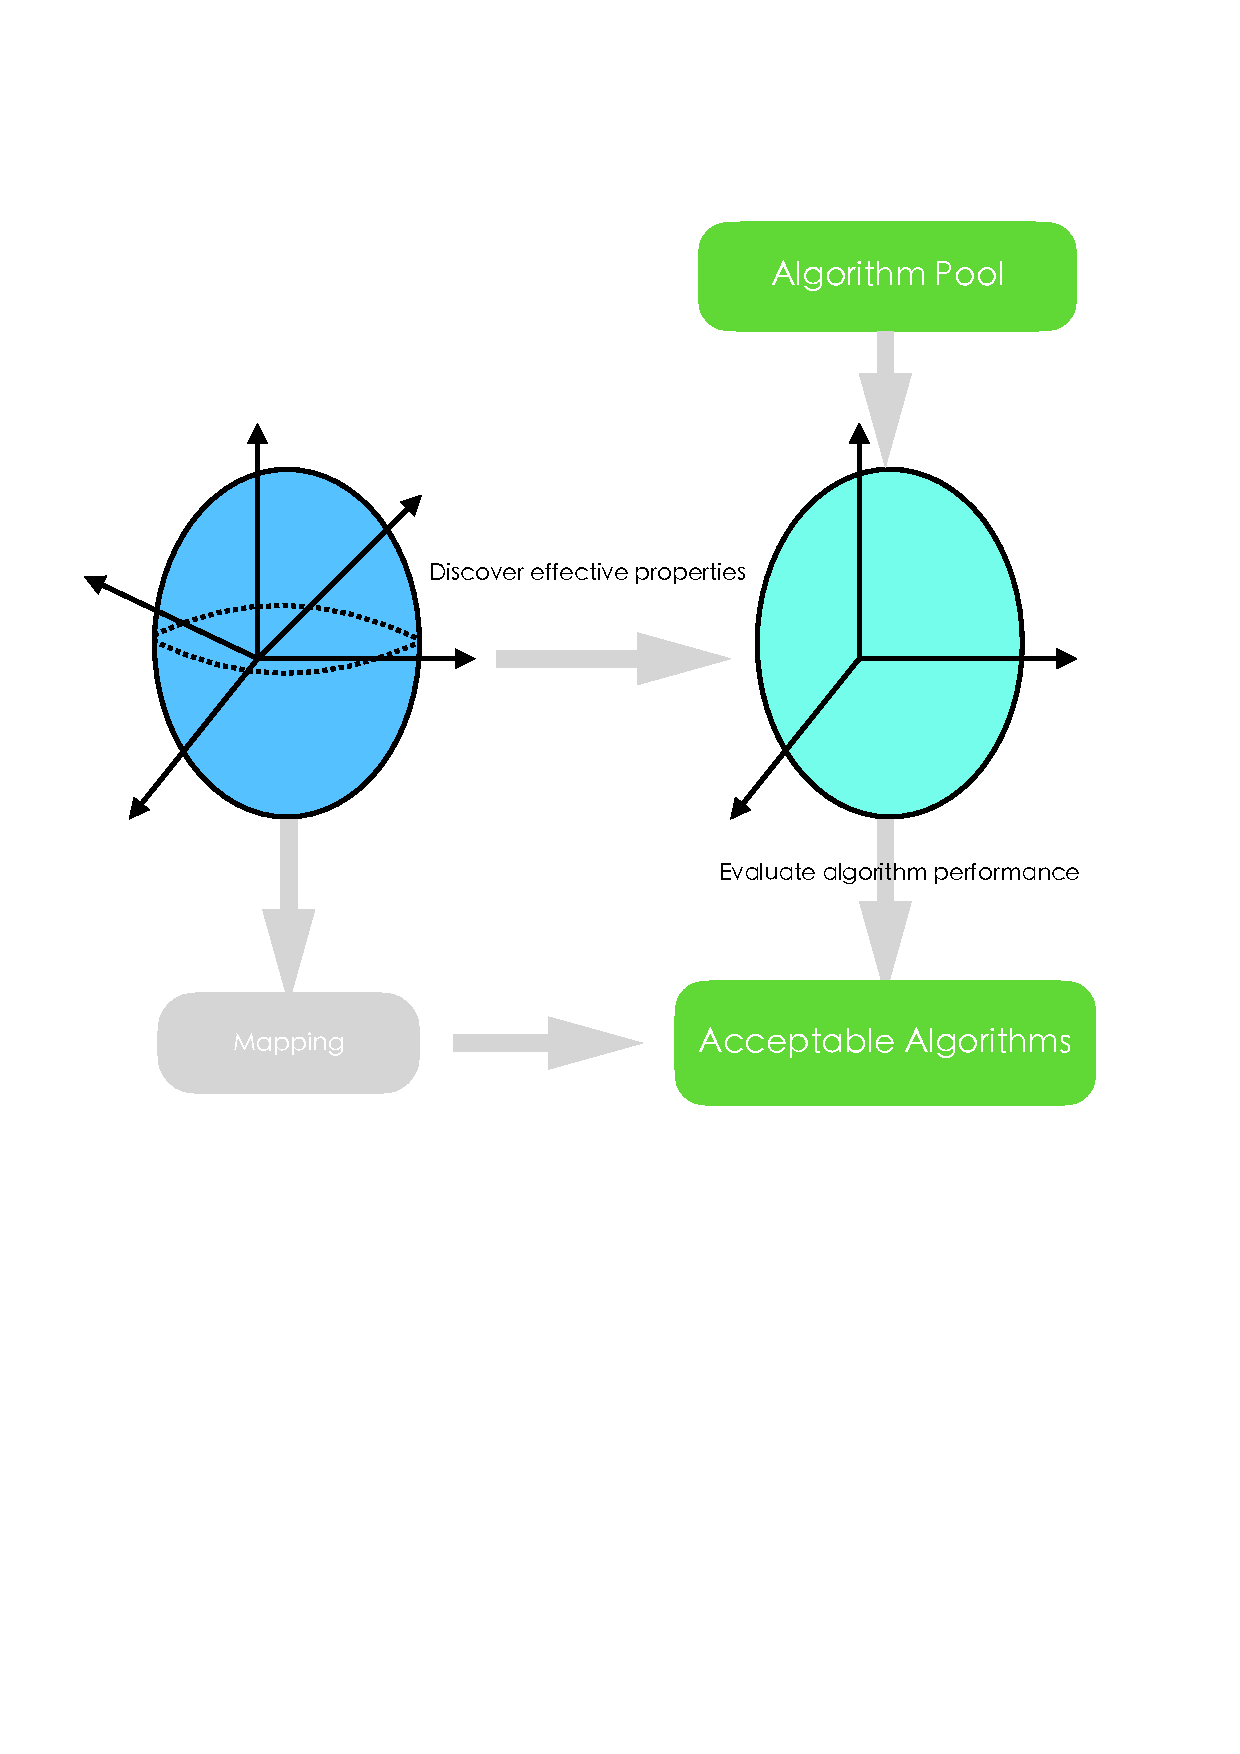
\includegraphics[width=0.8\textwidth]{images/mapping_3d_vision.pdf}
\end{figure}

% \begin{itemize}
% \item Establish the \textit{effective problem domain} (EPD): cope with large variation in material and shape.
% \item Evaluate algorithmic performance within EPD
% \item Derive mapping from problem conditions to algorithms.
% \end{itemize}

\end{frame}

%------------------------------------------------
\begin{frame}
\frametitle{Mapping: algorithms and baseline}

\begin{table}[!htbp]
\centering
\begin{tabular}{p{4cm}|c|c|c|c}
\toprule
Technique & Texture & Albedeo & Specular & Roughness\\
\midrule
PMVS: patch-based, seed points propagation MVS. & High & - & Low & -\\
\midrule
EPS: example-based Photometric Stereo & - & High & Low & High \\
\midrule
GSL: Gray-code Structured Light technique & - & High & Low & High\\
\midrule\midrule
VH: volumetric Visual Hull. & - & - & - & -\\
\midrule
LLS-PS: linear least squares Photometric Stereo. & - & High & Low & High\\
\bottomrule
\end{tabular}
\caption{Summary of the selected and baseline algorithms.}
\end{table}

\end{frame}

%------------------------------------------------
\begin{frame}
\frametitle{Mapping: quantitative measures and criteria}

\begin{itemize}
\item accuracy: the distance $d$ such that $X\%$ of the points on $R$ are within distance $d$ of $G$ is considered as accuracy;
\item completeness: the percentage of $G$ that is reconstructed by $R$;
\item angular error: angle between the estimated and ground truth normal, \textit{i.e.,} $arccos(n_g^T n)$.
\end{itemize}

\begin{figure}[!htbp]
\begin{tabular}{cc}
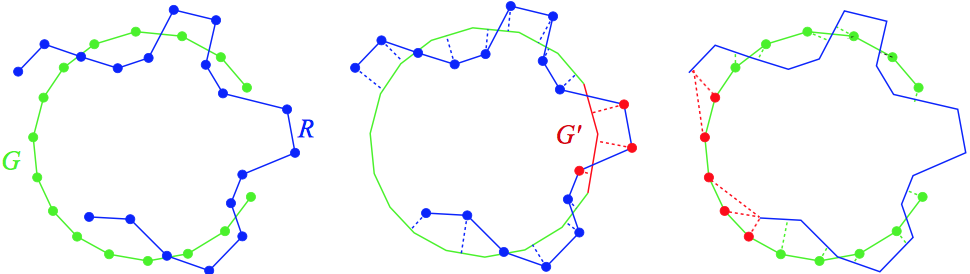
\includegraphics[width=0.6\textwidth]{mapping/qm_acc_cmp} &
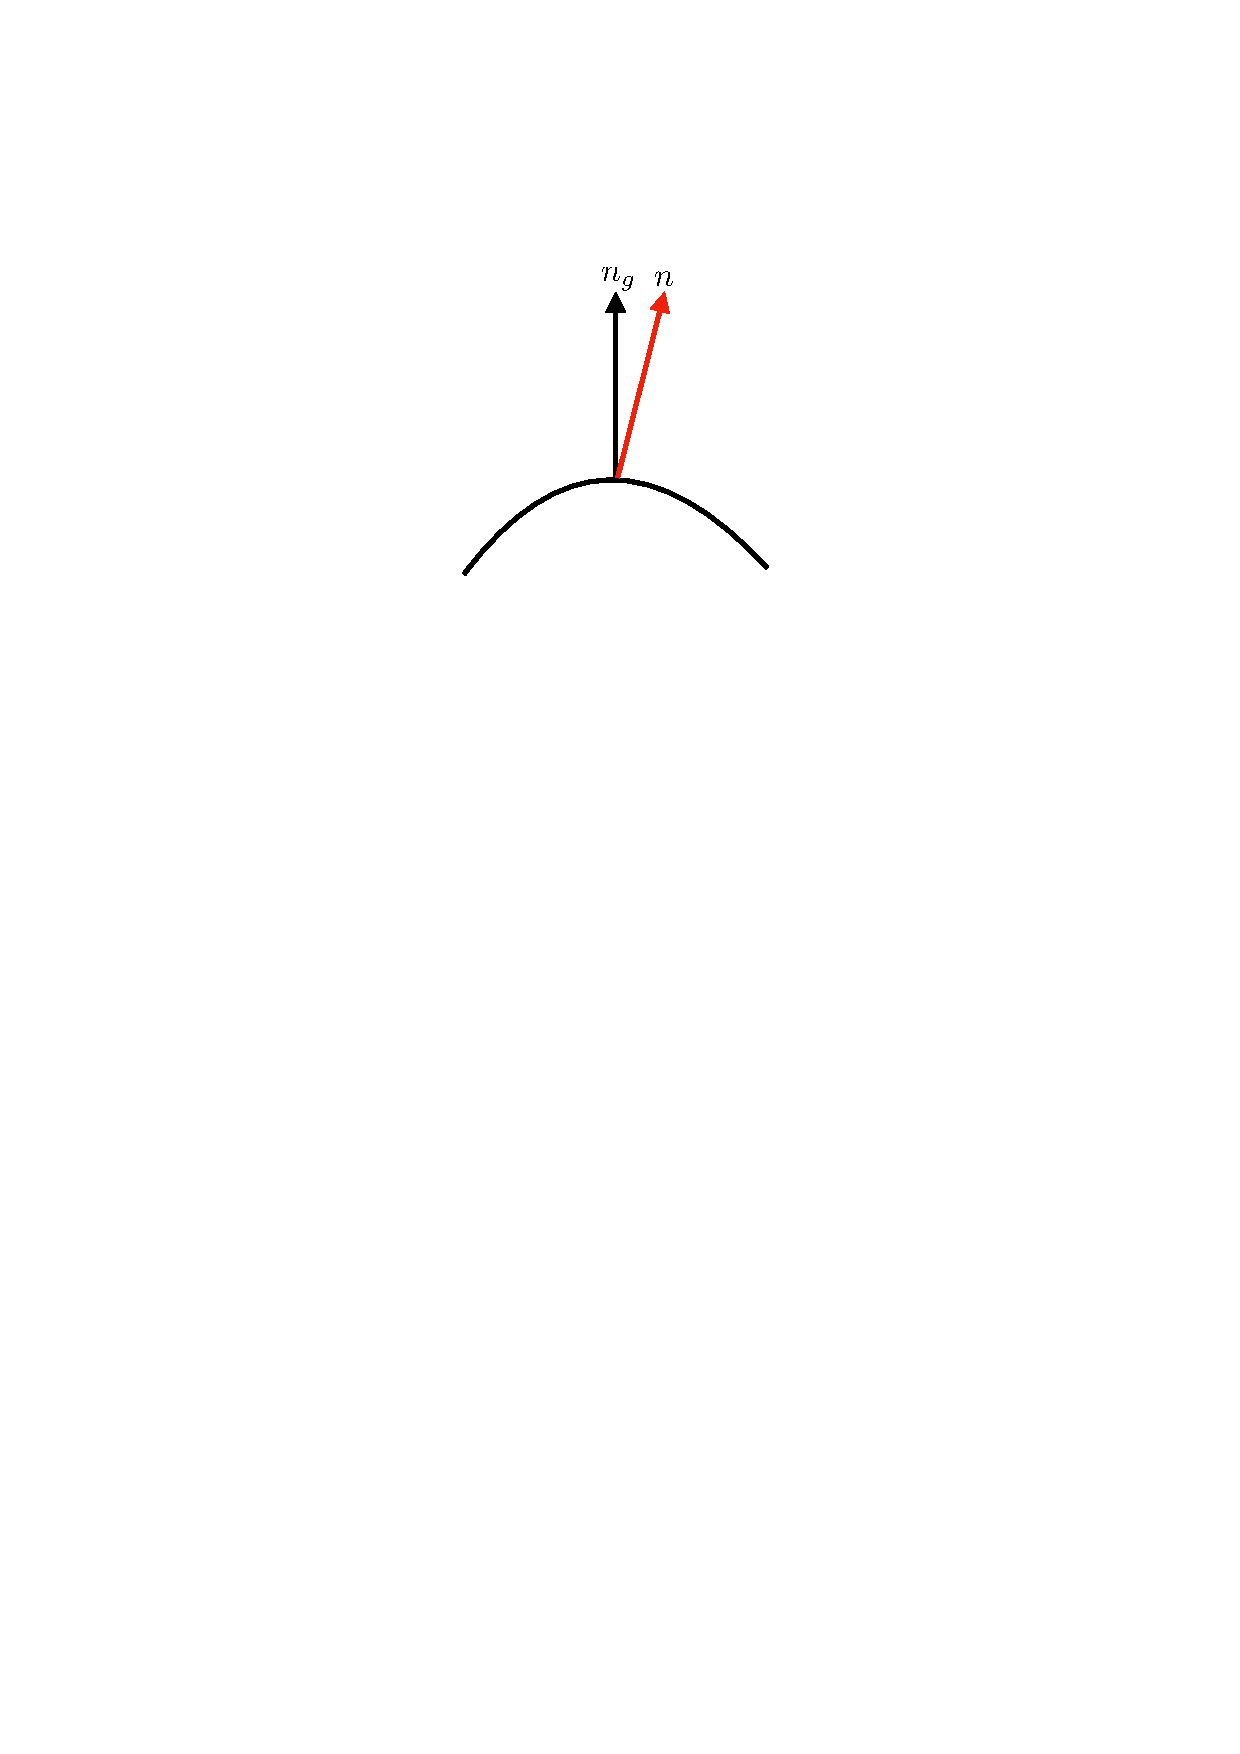
\includegraphics[width=0.17\textwidth]{mapping/qm_ang_error}\\
Accuracy and completeness & angular error
\end{tabular}
\end{figure}

\end{frame}

% %------------------------------------------------
% \begin{frame}
% \frametitle{Mapping: EPD of PMVS}

% \begin{table}[!htbp]
%   \centering
%   \caption{Problem conditions for establishing the \textit{effective problem domain} of PMVS.}
%   \begin{tabular}{l*{4}{c}}
%   \hline
%   \textbf{Cond} & Texture & Albedo & Specular & Roughness\\
%   \hline
%   \textbf{(a)} & [0.2, 0.8] & [0.2, 0.8] & 0.0 & 0.0\\
%   \textbf{(b)} & [0.2, 0.8] & 0.8 & [0.2, 0.8] & 0.0\\
%   \textbf{(c)} & [0.2, 0.8] & 0.8 & 0.0 & [0.2, 0.8]\\
%   \textbf{(d)} & 0.8 & [0.2, 0.8] & [0.2, 0.8] & 0.0\\
%   \textbf{(e)} & 0.8 & [0.2, 0.8] & 0.0 & [0.2, 0.8]\\
%   \textbf{(f)} & 0.8 & 0.8 & [0.2, 0.8] & [0.2, 0.8]\\
%   \hline
%   \end{tabular}
% \end{table}

% \textbf{Cond. (a). Texture and Albedo}
% \begin{figure}[!htbp]
% \includegraphics[width=0.3\textwidth]{mapping/depend_check/mvs_tex_alb}
% \end{figure}

% \end{frame}

% %------------------------------------------------
% \begin{frame}
% \frametitle{Mapping: EPD of PMVS (cont'd)}

% \textbf{Cond. (b). Texture and Specularity}
% \begin{figure}[!htbp]
% \begin{tabular}{cc}
% \includegraphics[width=0.22\textwidth]{mapping/depend_check/mvs_tex_spec}&
% 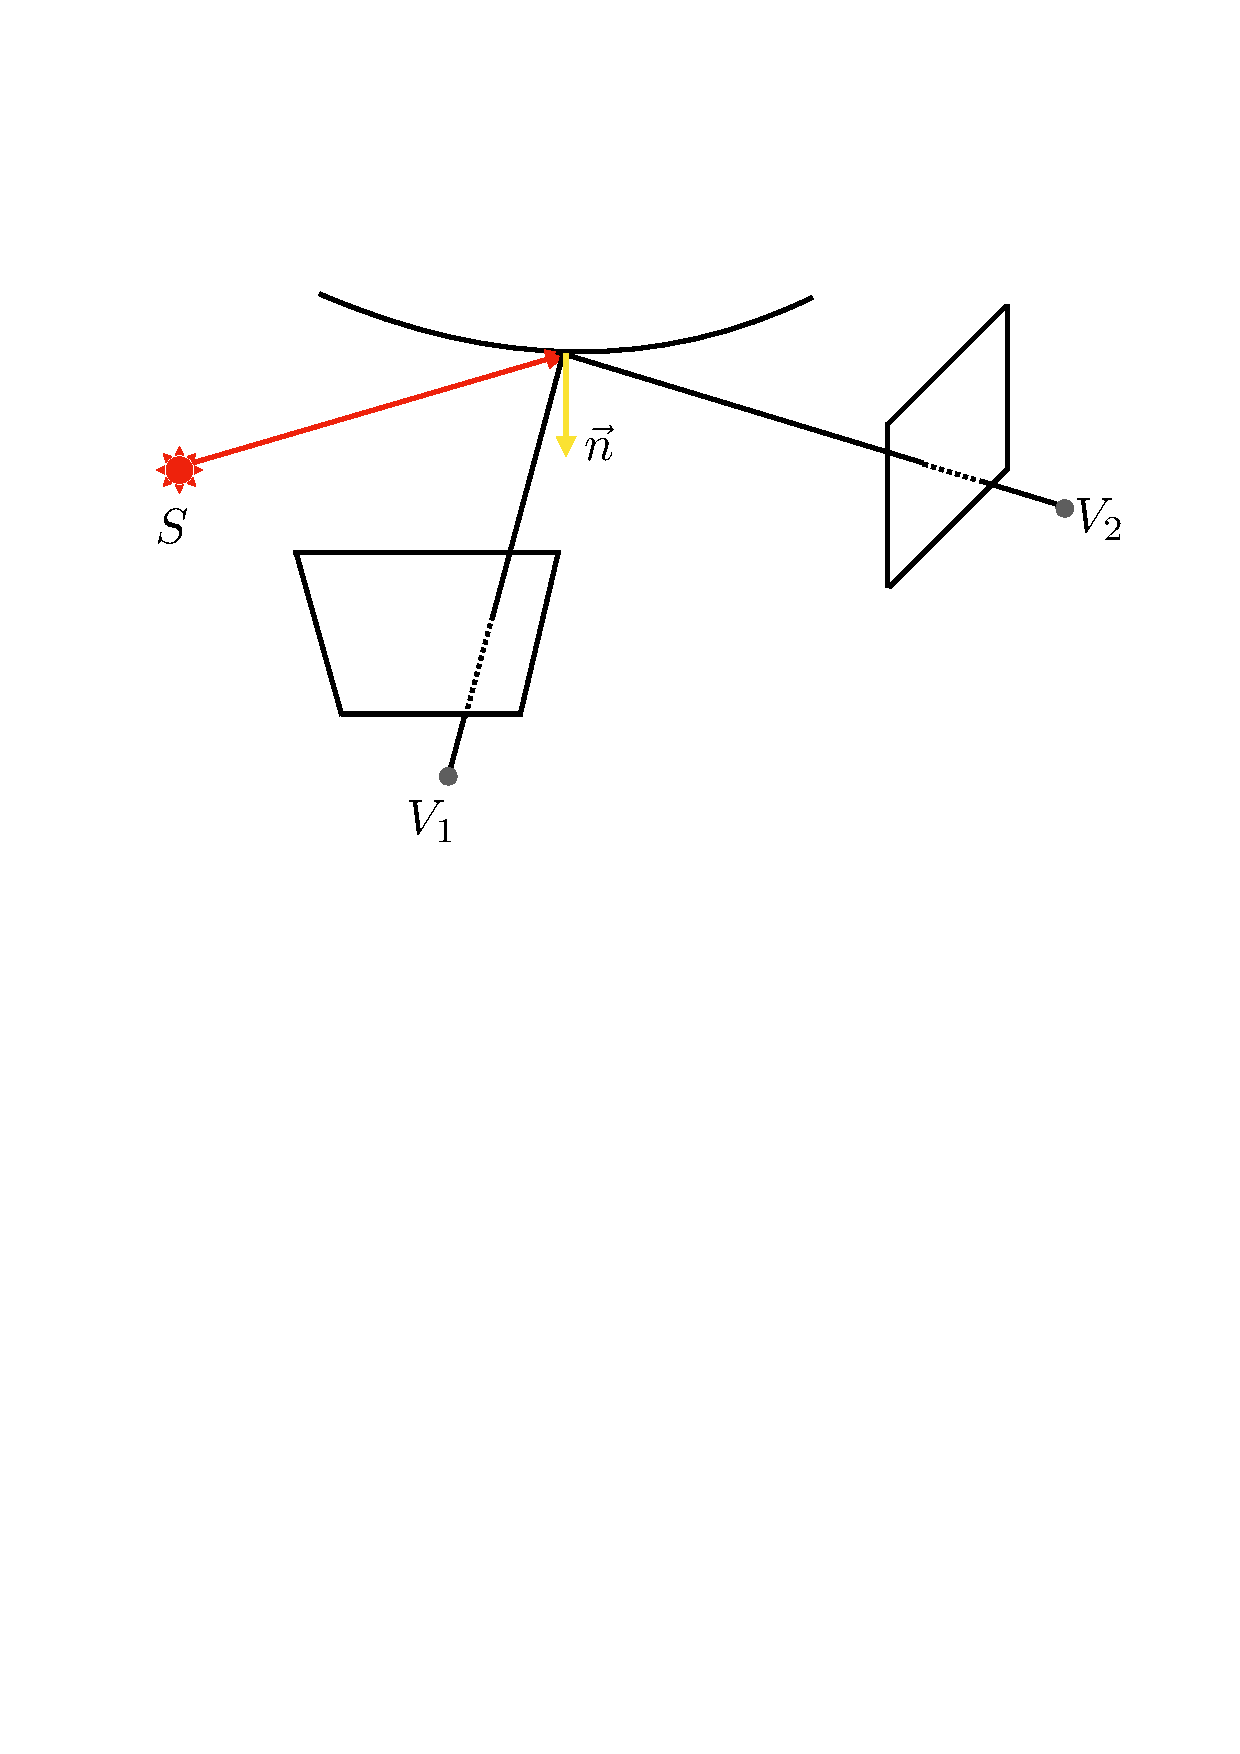
\includegraphics[width=0.22\textwidth]{mapping/mvs_spec/mvs_spec}\\
% (a). Algo. performance & (b) Image formation\\
% 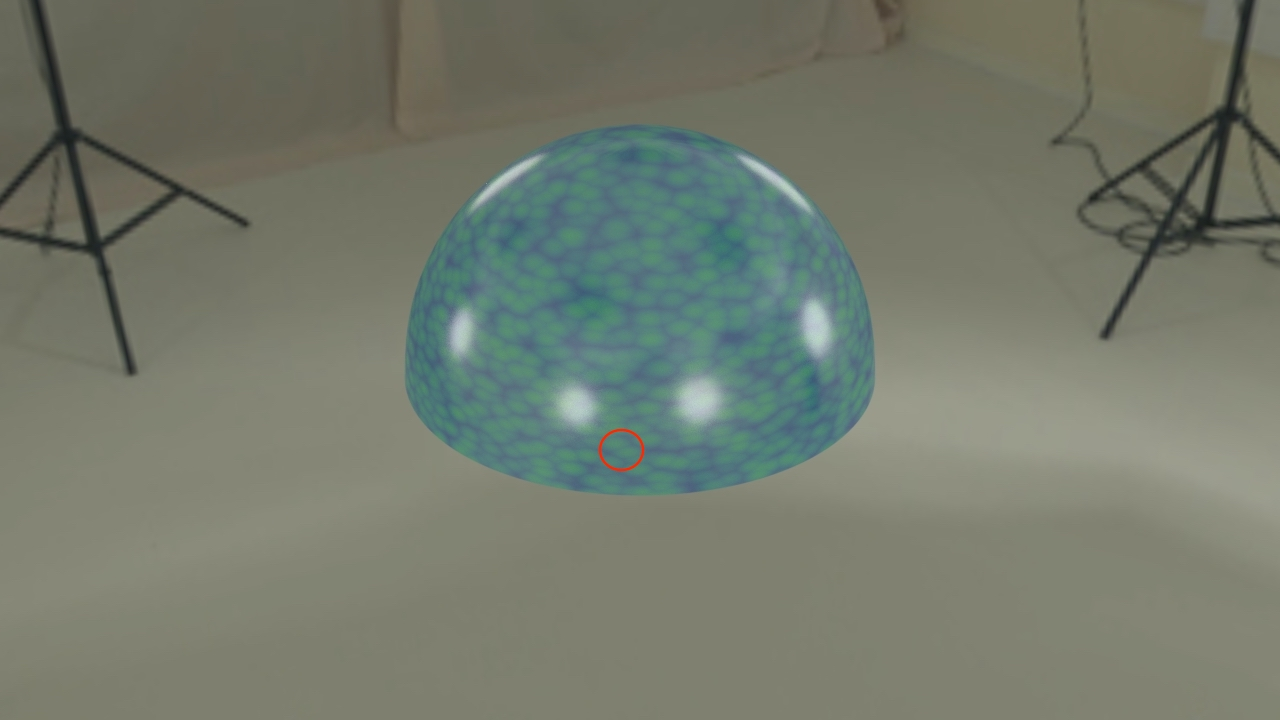
\includegraphics[width=0.22\textwidth]{mapping/mvs_spec/mvs_spec_01}&
% 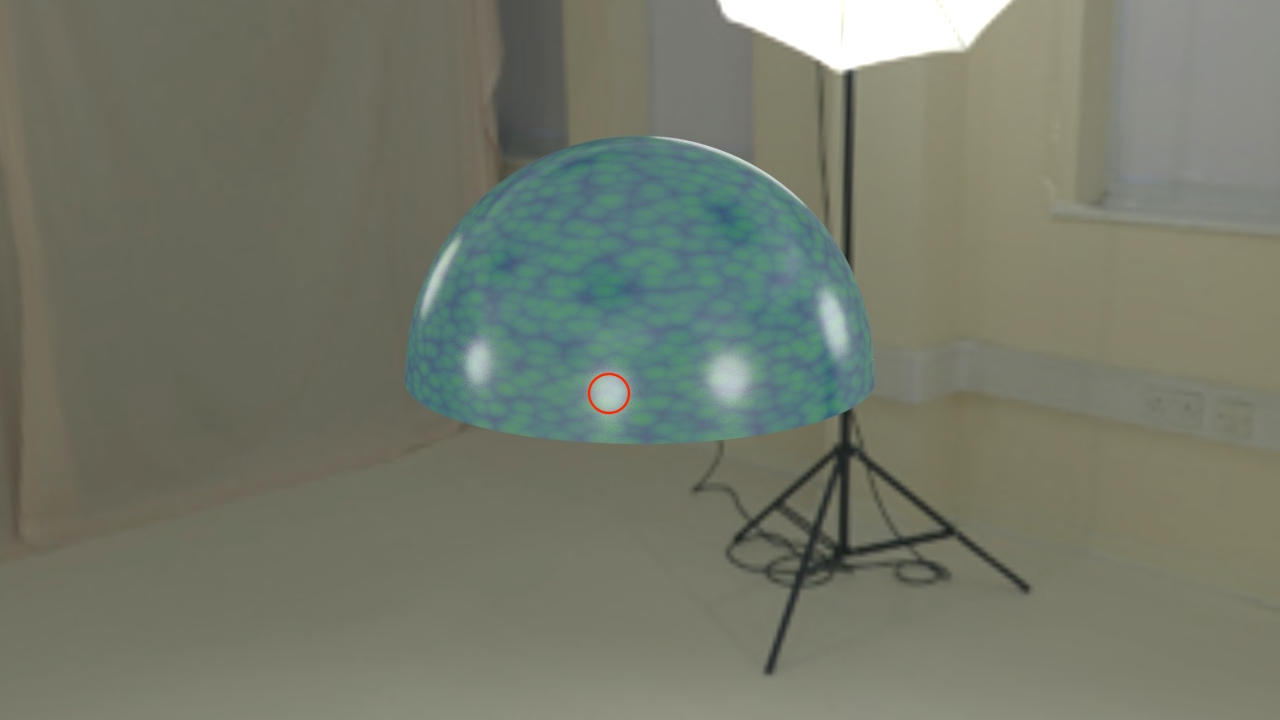
\includegraphics[width=0.22\textwidth]{mapping/mvs_spec/mvs_spec_00}\\
% (c) $V_1$ & (d) $V_2$\\
% \end{tabular}
% \caption{(a) shows the algorithm performance w.r.t. texture and specularity. (b) shows the reflection of light off a specular surface. $V_1$ received the diffuse component while $V_2$ receives the specular component. (c), (d) shows the images observed from these two views. The specular area (red circle) observed in $V_2$ is visible in $V_1$.}
% \end{figure}

% \end{frame}

% %------------------------------------------------
% \begin{frame}
% \frametitle{Mapping: EPD of PMVS (cont'd)}

% \textbf{Cond. (d). Albedo and Specularity}
% \begin{figure}
% \centering
% \begin{tabular}{ccc}
% \multirow{2}{*}{
%   \includegraphics[width=0.25\textwidth]{mapping/depend_check/mvs_alb_spec}
%   }
% &
% 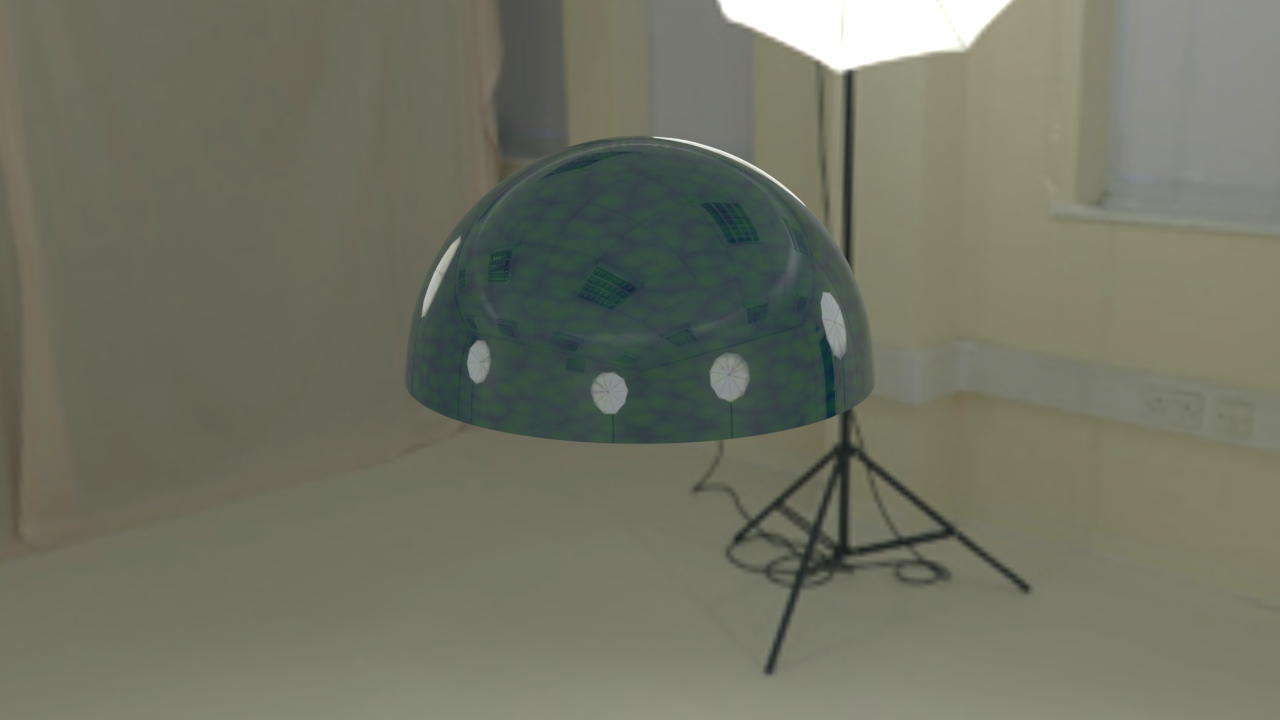
\includegraphics[width=0.22\textwidth]{mapping/mvs_alb_spec/alb_spec_0202}&
% % 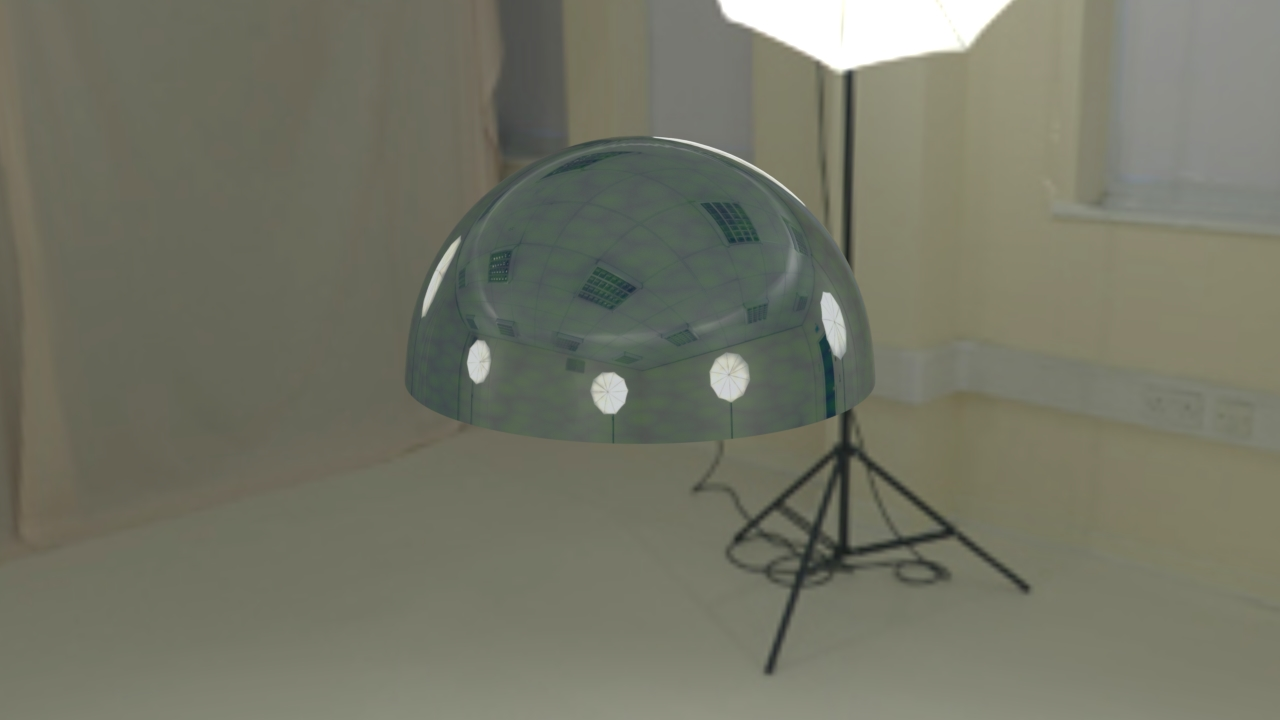
\includegraphics[width=0.2\textwidth]{mapping/mvs_alb_spec/alb_spec_0205}&
% 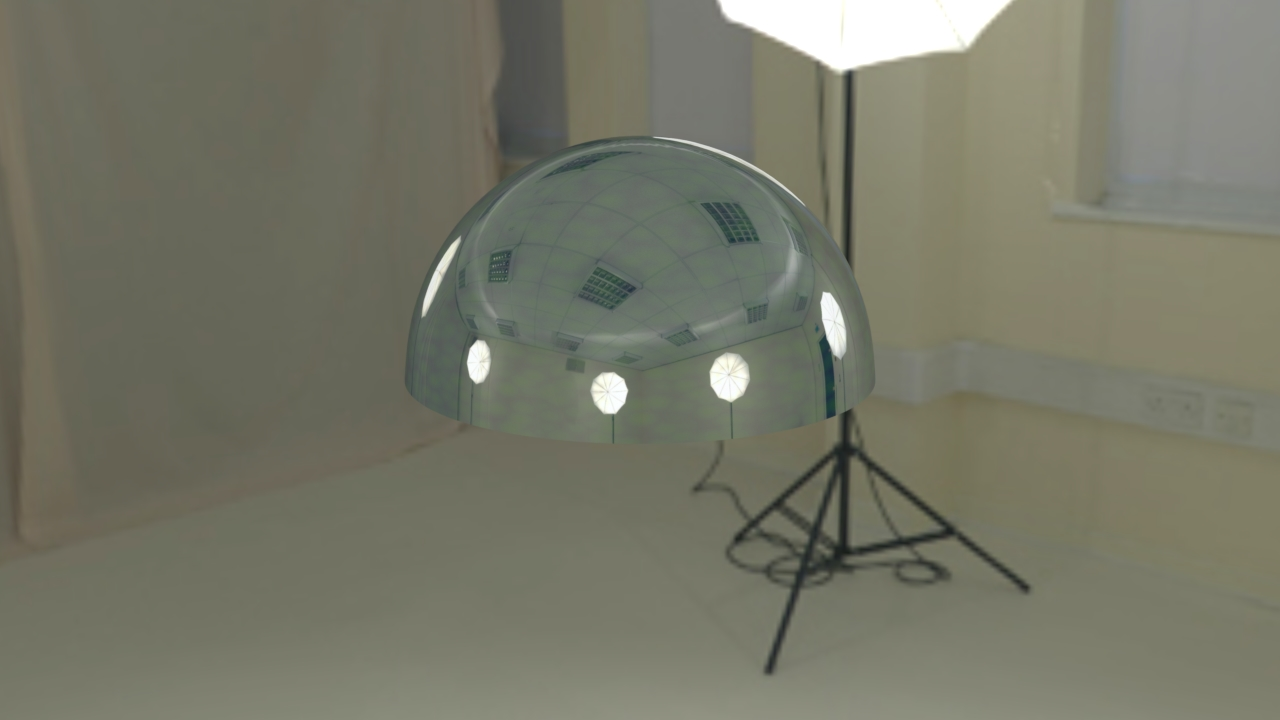
\includegraphics[width=0.22\textwidth]{mapping/mvs_alb_spec/alb_spec_0208}\\
% & (a) spec: 0.2 & (b) spec: 0.8\\
% &
% 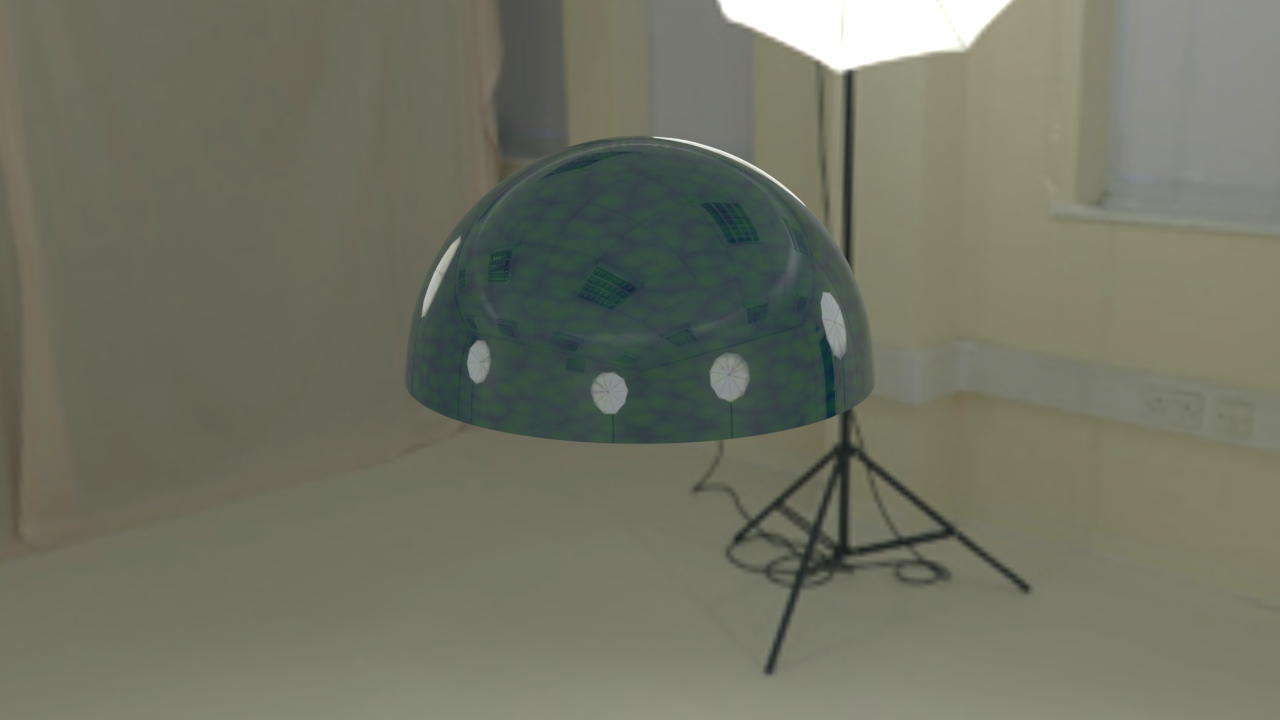
\includegraphics[width=0.22\textwidth]{mapping/mvs_alb_spec/alb_spec_0202}&
% % 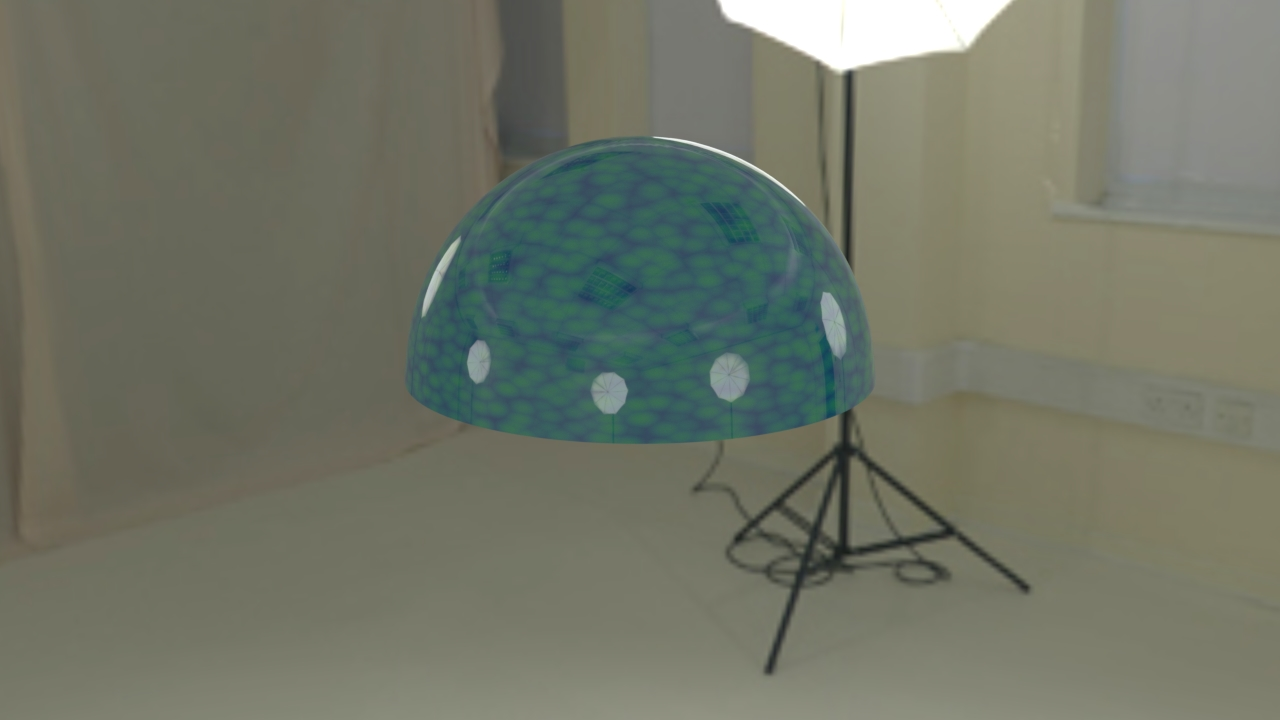
\includegraphics[width=0.2\textwidth]{mapping/mvs_alb_spec/alb_spec_0502}&
% 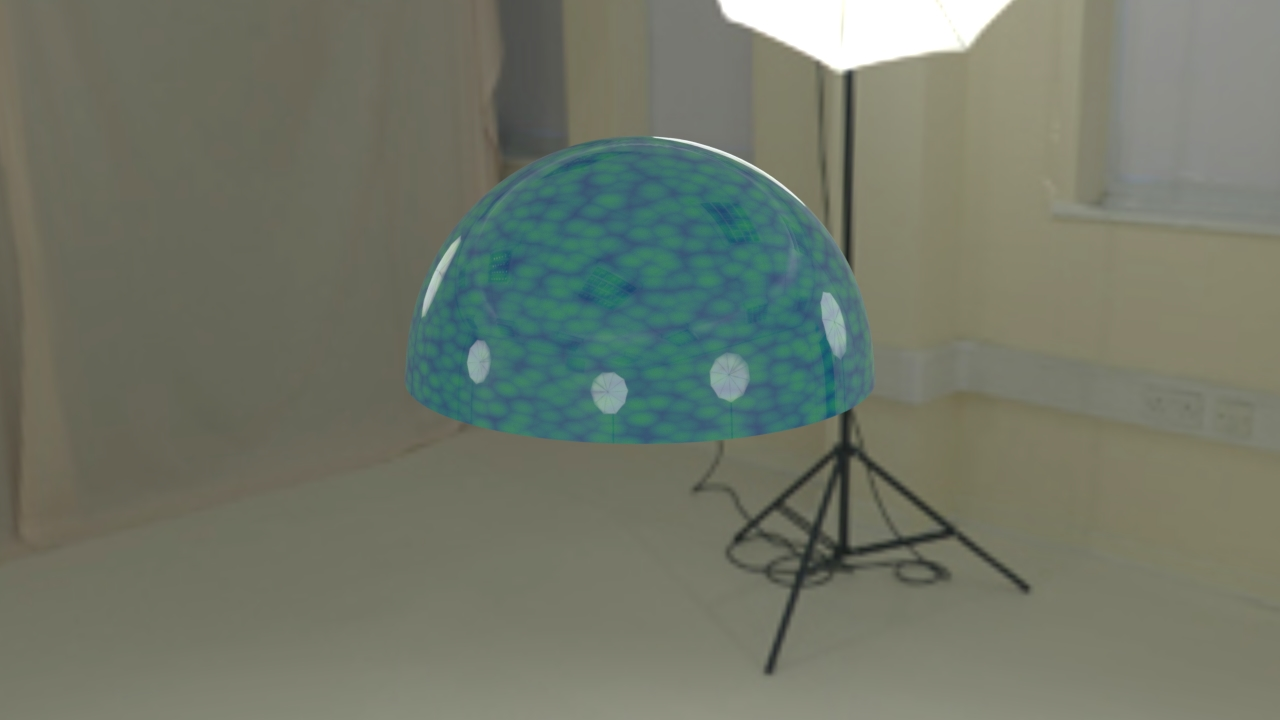
\includegraphics[width=0.22\textwidth]{mapping/mvs_alb_spec/alb_spec_0802}\\
% & (c) alb: 0.2 & (d) alb: 0.8\\
% \end{tabular}
% % \caption{(a)-(b). The albedo is set as 0.2, (c)-(d). The specularity is set as 0.2. According to energy conservation, as the specular component increases, the diffuse component decreases.}
% \caption{The law of conservation of energy demands that as the specular reflection increases, the diffuse reflection decreases.}
% \end{figure}

% \end{frame}

% %------------------------------------------------
% \begin{frame}
% \frametitle{Mapping: \textit{effective properties} of PMVS}

% \begin{table}[!htbp]
%   \centering
%   \begin{tabular}{l*{4}{c}}
%   \hline
%   \textbf{Metric} & Texture & Albedo & Specular & Roughness\\
%   \hline
%   Accuracy & \checkmark & \checkmark & \checkmark & \ding{55}\\
%   Completeness & \checkmark & \checkmark & \checkmark & \ding{55}\\
%   \hline
%   \end{tabular}
%   \caption{The \textit{effective problem domain} of PMVS in terms of accuracy and completeness.}
% \end{table}

% \end{frame}

% %------------------------------------------------
% \begin{frame}
% \frametitle{Mapping: mapping construction}

% \begin{itemize}
% \item Accuracy and completeness improves consistently as the \textit{texture} level increases. 
% \item Accuracy and completeness results deteriorate consistently as \textit{specularity} increases, and this negative impact is most significant when texture level is medium or albedo value is low. 
% \item The effect of \textit{albedo} on a surface with low texture is negligible. However, albedo has a noticeably more significant positive impact on completeness as the texture of a specular surface increases.
% \end{itemize}

% \begin{figure}[!htbp]
% \begin{tabular}{ccc}
% \includegraphics[width=0.25\textwidth]{mapping/training/mvs_train_spec_02}&
% \includegraphics[width=0.25\textwidth]{mapping/training/mvs_train_spec_05}&
% \includegraphics[width=0.25\textwidth]{mapping/training/mvs_train_spec_08}\\
% % (a) & (b) & (c)\\
% % \includegraphics[width=0.25\textwidth]{mapping/training/mvs_train_tex_02}&
% % \includegraphics[width=0.25\textwidth]{mapping/training/mvs_train_tex_05}&
% % \includegraphics[width=0.25\textwidth]{mapping/training/mvs_train_tex_08}\\
% % (d) & (e) & (f)\\
% % \includegraphics[width=0.25\textwidth]{mapping/training/mvs_train_alb_02}&
% % \includegraphics[width=0.25\textwidth]{mapping/training/mvs_train_alb_05}&
% % \includegraphics[width=0.25\textwidth]{mapping/training/mvs_train_alb_08}\\
% % (g) & (h) & (i)\\
% \end{tabular}
% \end{figure}

% \end{frame}

% %------------------------------------------------
% \begin{frame}
% \frametitle{Mapping: mapping construction (cont'd)}

% \begin{table}[!htbp]
%   \centering
%   \begin{tabular}{l*{4}{c}}
%   \toprule
%   \textbf{Metric} & Texture & Albedo & Specular & Roughness\\
%   \midrule
%   Accuracy & 0.5 & 0.5 & 0.2 & -\\
%   \&Completeness & 0.5 & 0.8 & 0.2 & -\\
%            & 0.5 & 0.8 & 0.5 & -\\
%            & 0.8 & 0.2 & 0.2 & -\\
%            & 0.8 & 0.5 & 0.2 & -\\
%            & 0.8 & 0.8 & 0.2 & -\\
%            & 0.8 & 0.5 & 0.5 & -\\
%            & 0.8 & 0.8 & 0.5 & -\\
%            & 0.8 & 0.5 & 0.8 & -\\
%            & 0.8 & 0.8 & 0.8 & -\\
%   \bottomrule
%   \end{tabular}
%   \caption{The working problem conditions of PMVS in terms of the two metrics \textit{accuracy} and \textit{completeness}.}
%   \label{tab:mvs_training_result}
% \end{table}

% \end{frame}

%------------------------------------------------
\section{Evaluation of Interface}
%------------------------------------------------
\begin{frame}
\tableofcontents[currentsection,currentsubsection, 
    hideothersubsections, 
    sectionstyle=show/shaded,]
\end{frame}

%------------------------------------------------
\begin{frame}
\frametitle{Interpretation: Key Evaluation Questions}

\begin{itemize}
\item Evaluation of mapping: is the mapping robust to changes of shape?
\item Evaluation of interpreter: can the proof-of-concept interpreter return a successful reconstruction given the correct description?
\end{itemize}

\end{frame}

%------------------------------------------------
\begin{frame}
\frametitle{Interpretation: evaluation of mapping}

\begin{itemize}
\item Shape variation: too vast and complicated to model;
\item Instead focus on one geometric property: surface concavity, and see how robust is the mapping with respect to concavity changes.
\end{itemize}


\end{frame}

%------------------------------------------------
\begin{frame}
\frametitle{Interpretation: evaluation of mapping (cont'd)}

\begin{figure}[!htbp]
\centering
\begin{tabular}{*{4}{c}}
  \toprule
  Quantitative results & ~ & Qualitative results & ~\\
  \midrule
  \includegraphics[width=0.2\textwidth]{interp/synth_data/bottle/bottle_08080208}&
  \fcolorbox{green}{white}{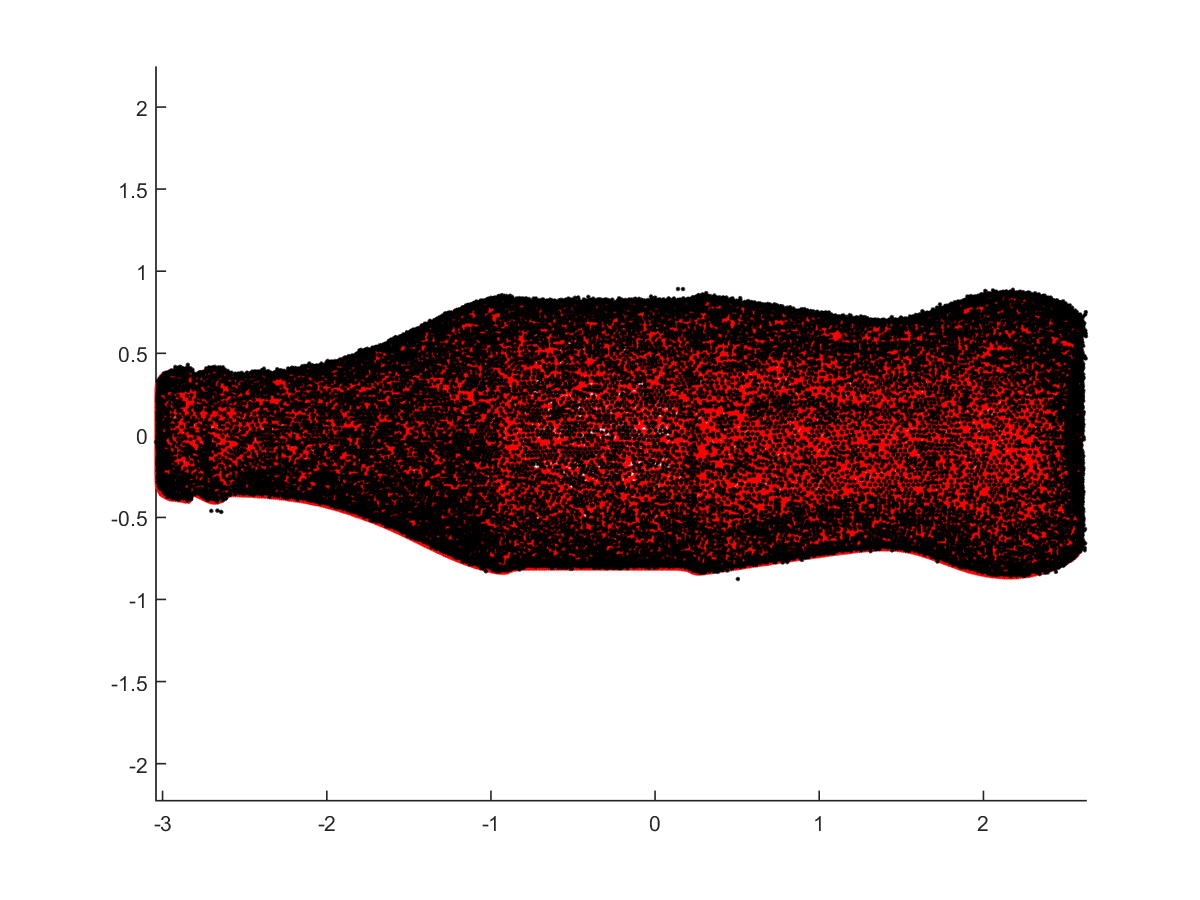
\includegraphics[width=0.15\textwidth]{interp/synth_data/bottle/bottle_mvs_08080208.png}}&
  \fcolorbox{green}{white}{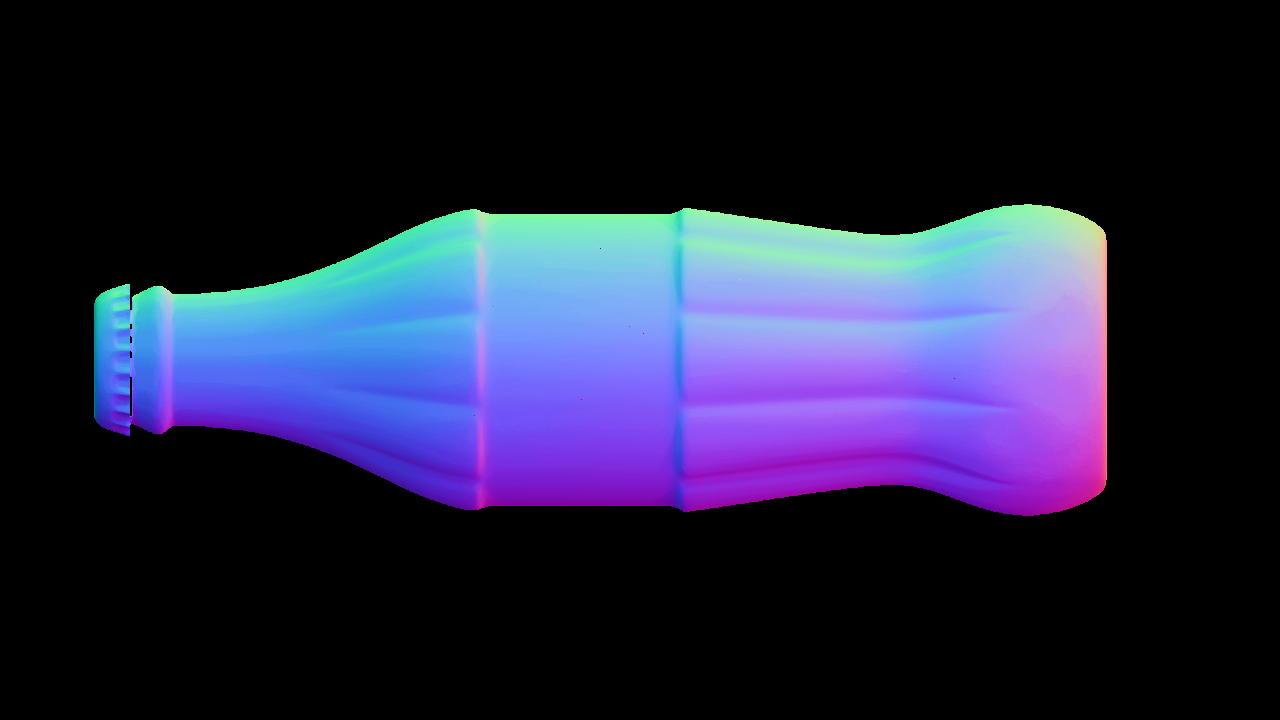
\includegraphics[width=0.2\textwidth]{interp/synth_data/bottle/bottle_ps_08080208.png}}&
  \fcolorbox{green}{white}{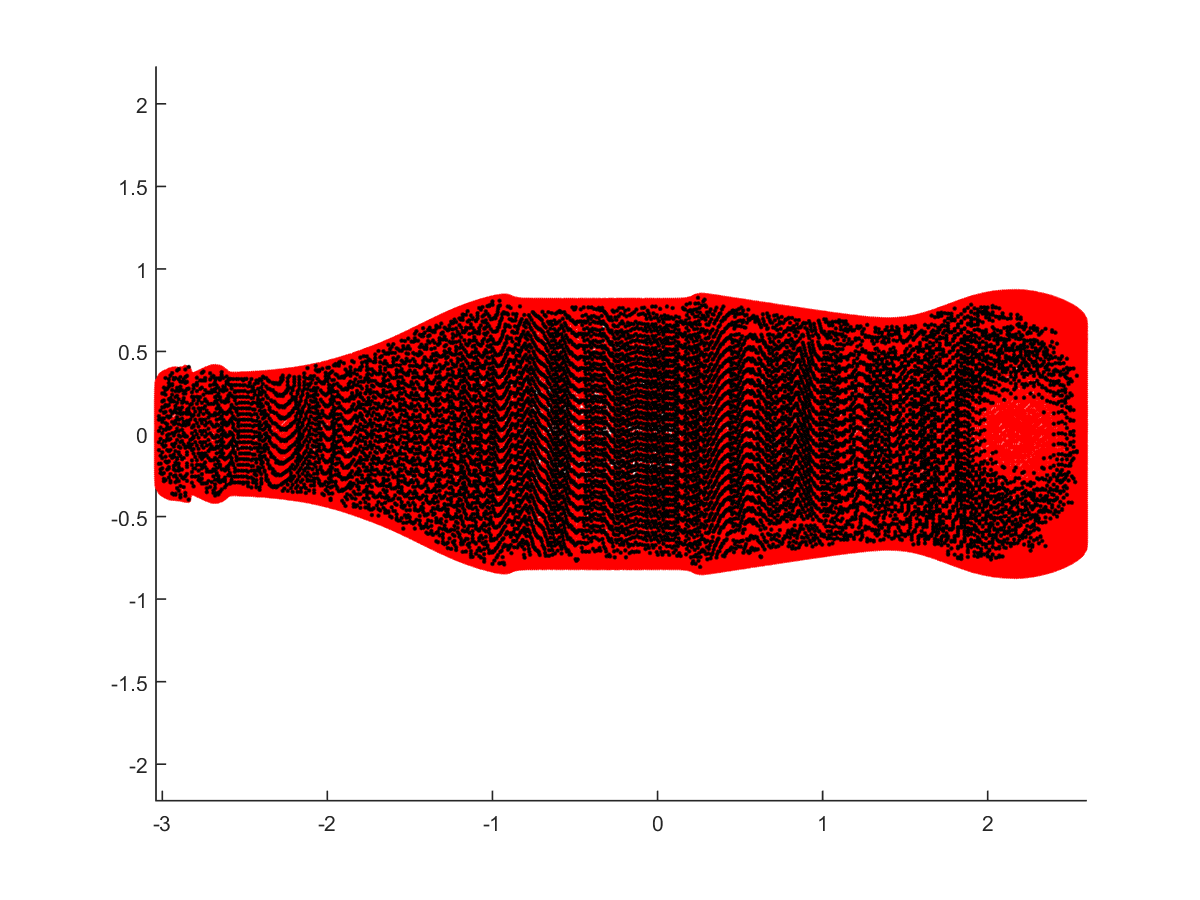
\includegraphics[width=0.15\textwidth]{interp/synth_data/bottle/bottle_sl_08080208.png}}\\
  \includegraphics[width=0.2\textwidth]{interp/synth_data/knight/knight_08080208}&
  \fcolorbox{green}{white}{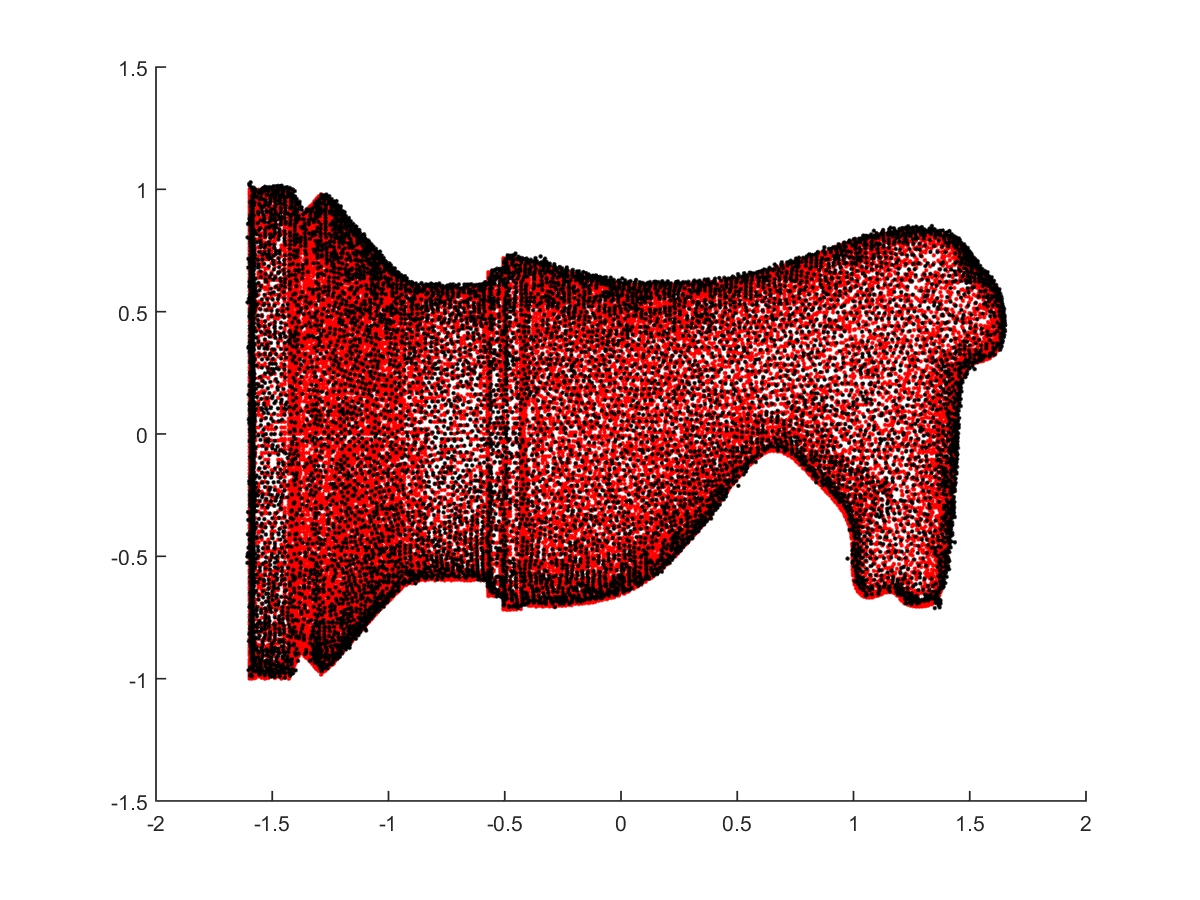
\includegraphics[width=0.15\textwidth]{interp/synth_data/knight/knight_mvs_08080208.png}}&
  \fcolorbox{green}{white}{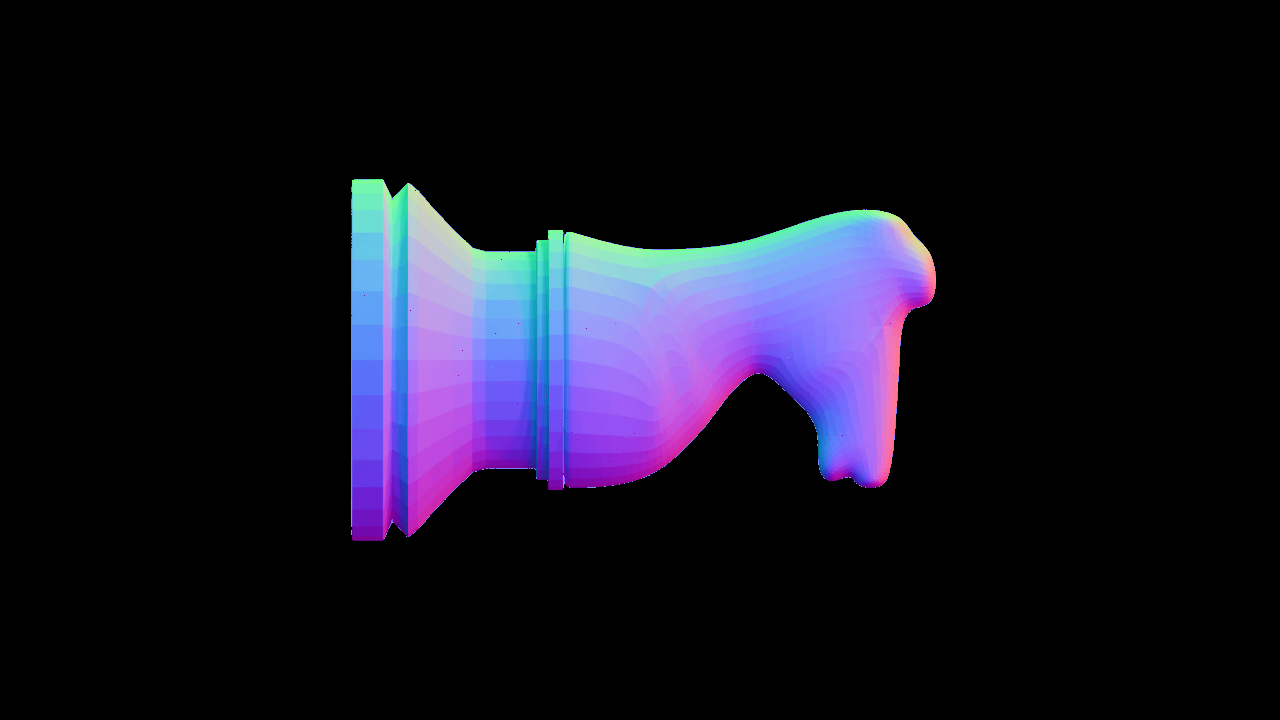
\includegraphics[width=0.2\textwidth]{interp/synth_data/knight/knight_ps_08080208.png}}&
  \fcolorbox{green}{white}{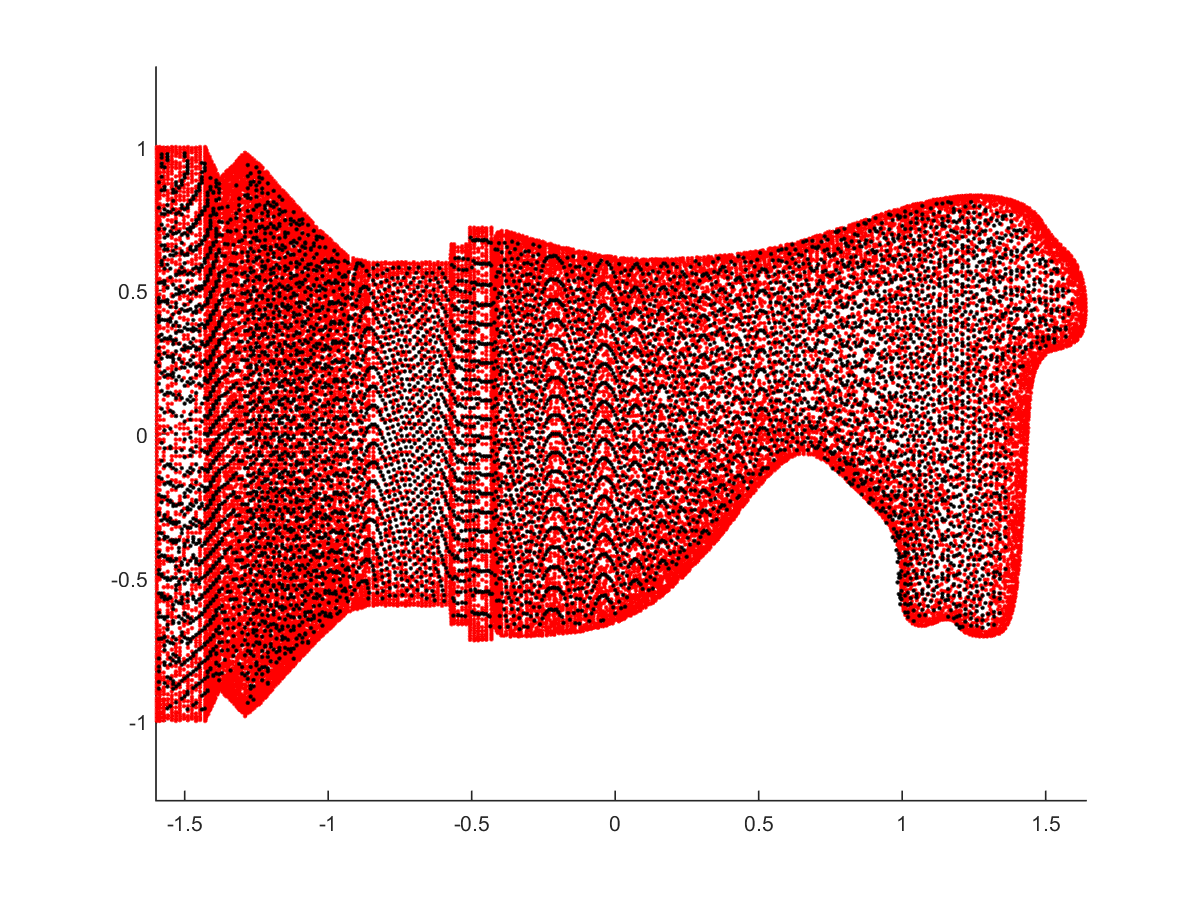
\includegraphics[width=0.15\textwidth]{interp/synth_data/knight/knight_sl_08080208.png}}\\
  \includegraphics[width=0.2\textwidth]{interp/synth_data/king/king_08080208}&
  \fcolorbox{green}{white}{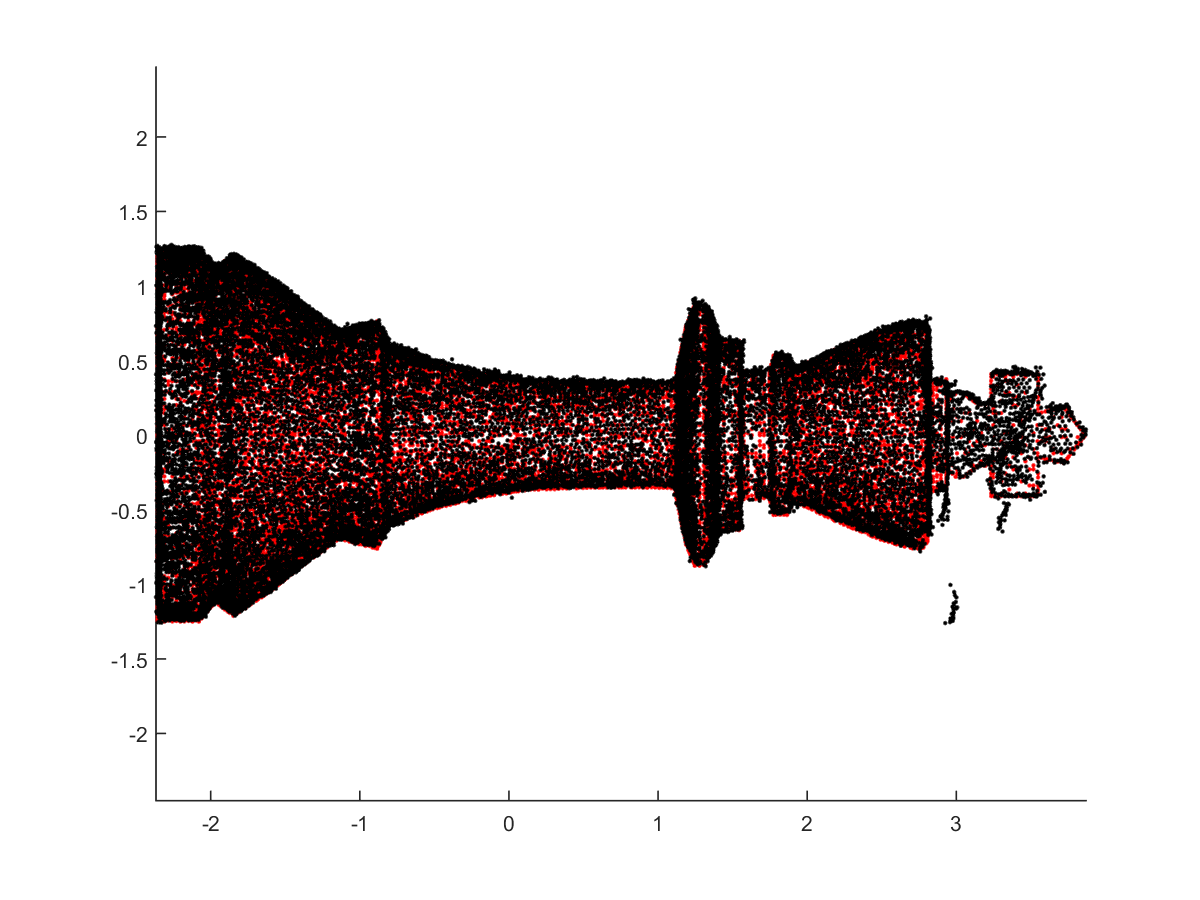
\includegraphics[width=0.15\textwidth]{interp/synth_data/king/king_mvs_08080208.png}}&
  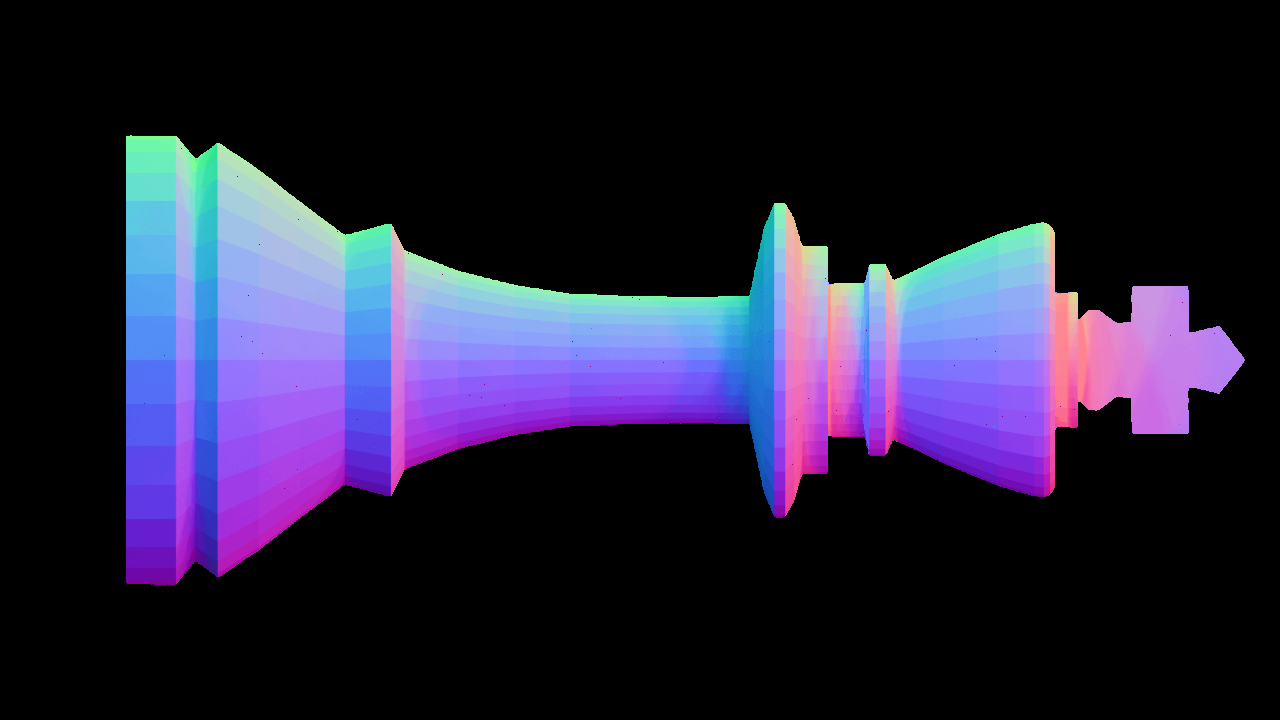
\includegraphics[width=0.2\textwidth]{interp/synth_data/king/king_ps_08080208.png}&
  \fcolorbox{green}{white}{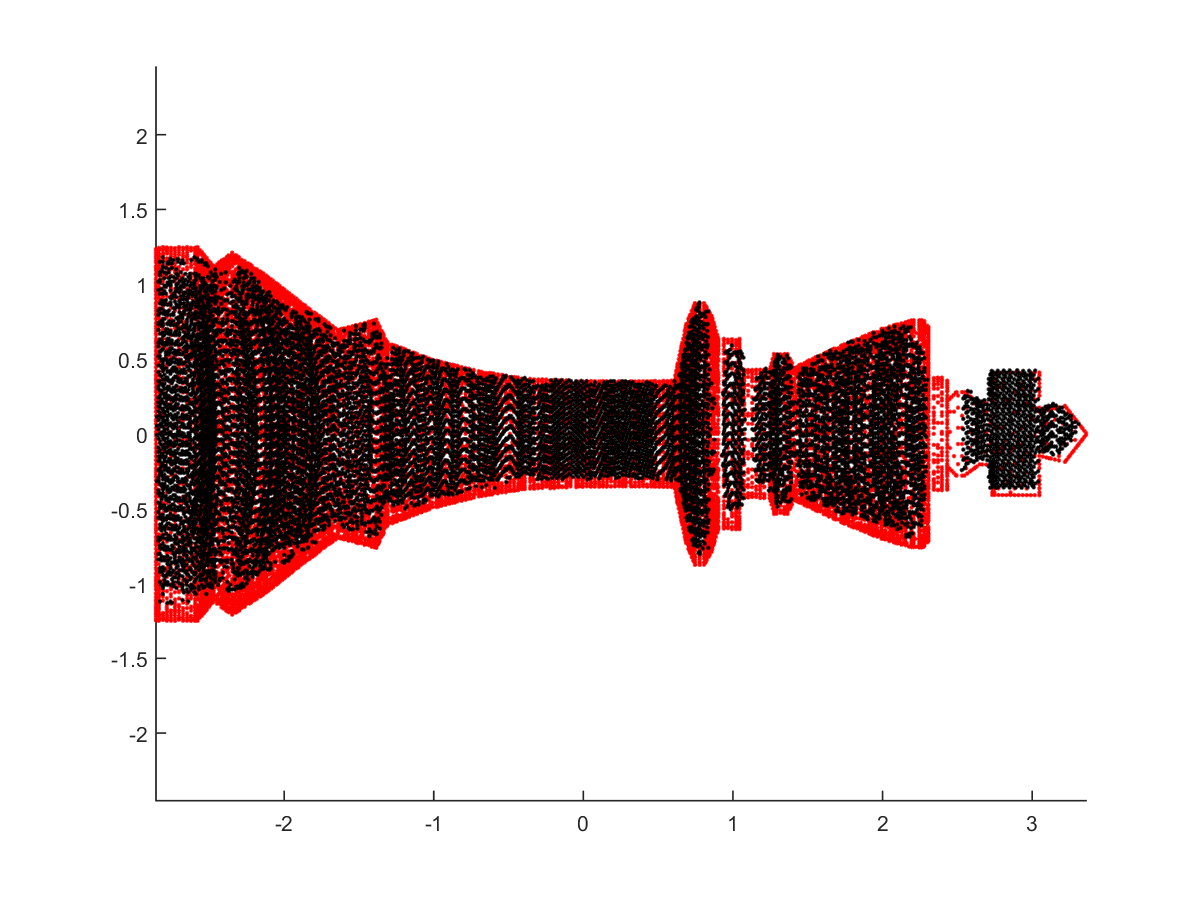
\includegraphics[width=0.15\textwidth]{interp/synth_data/king/king_sl_08080208.png}}\\
  \bottomrule
  ~ & PMVS & EPS & GSL\\
\end{tabular}
\caption{Problem condition: 08080208, mapped algorithms: PMVS, EPS, GSL.}
\end{figure}

\end{frame}

%------------------------------------------------
\begin{frame}
\frametitle{Interpretation: evaluation of mapping (cont'd)}

Conclusion:
\begin{itemize}
\item Mappings to PMVS and GSL are robust to concavity changes whereas those to EPS are not.
\end{itemize}

Suggestions:
\begin{itemize}
\item Develop more advanced description, incorporating concavity into the description
\item Use more underlying algorithms that are robust to concavity changes.
\end{itemize}

\end{frame}

%------------------------------------------------
\begin{frame}
\frametitle{Proof-of-concept interpreter}

An interpreter selects an appropriate algorithm based on description of problem condition and constraints.

\begin{figure}[!htbp]
\centering
\includegraphics[width=0.8\textwidth]{interp/interpreter.pdf}
\end{figure}

\end{frame}

%------------------------------------------------
\begin{frame}
\frametitle{Interpretation: evaluation of interpreter}

\begin{figure}[!htbp]
\centering
\begin{tabular}{lccccr}
\toprule
Desc \# & Bust & Vase1 & Barrel & Vase0 & Selected Algo.\\
\midrule
1 & 
\fcolorbox{green}{white}{\raisebox{-.5\height}{\includegraphics[width=0.1\textwidth]{interp/synth_interp/beethoven_sl}}}&
\raisebox{-.5\height}{\includegraphics[width=0.1\textwidth]{interp/synth_interp/vase0_sl}}&
\raisebox{-.5\height}{\includegraphics[width=0.1\textwidth]{interp/synth_interp/barrel_sl}}&
\raisebox{-.5\height}{\includegraphics[width=0.1\textwidth]{interp/synth_interp/vase2_sl}}&
GSL\\
2 & 
\raisebox{-.5\height}{\includegraphics[width=0.1\textwidth]{interp/synth_interp/beethoven_ps}}&
\fcolorbox{green}{white}{\raisebox{-.5\height}{\includegraphics[width=0.1\textwidth]{interp/synth_interp/vase0_ps}}}&
\raisebox{-.5\height}{\includegraphics[width=0.1\textwidth]{interp/synth_interp/barrel_ps}}&
\raisebox{-.5\height}{\includegraphics[width=0.1\textwidth]{interp/synth_interp/vase2_ps}}&
EPS\\
3 & 
\raisebox{-.5\height}{\includegraphics[width=0.1\textwidth]{interp/synth_interp/beethoven_sl}}&
\raisebox{-.5\height}{\includegraphics[width=0.1\textwidth]{interp/synth_interp/vase0_sl}}&
\fcolorbox{green}{white}{\raisebox{-.5\height}{\includegraphics[width=0.1\textwidth]{interp/synth_interp/barrel_sl}}}&
\raisebox{-.5\height}{\includegraphics[width=0.1\textwidth]{interp/synth_interp/vase2_sl}}&
GSL\\
4 &
\raisebox{-.5\height}{\includegraphics[width=0.1\textwidth]{interp/synth_interp/beethoven_mvs}}&
\raisebox{-.5\height}{\includegraphics[width=0.1\textwidth]{interp/synth_interp/vase0_mvs}}&
\raisebox{-.5\height}{\includegraphics[width=0.1\textwidth]{interp/synth_interp/barrel_mvs}}&
\fcolorbox{green}{white}{\raisebox{-.5\height}{\includegraphics[width=0.1\textwidth]{interp/synth_interp/vase2_mvs}}}&
PMVS\\
\bottomrule
\end{tabular}
\end{figure}

\end{frame}

%------------------------------------------------
\begin{frame}
\frametitle{Interpretation: real-world objects}

\begin{figure}[!htbp]
\centering
\begin{tabular}{c|*{4}{p{2cm}}}
\toprule
class \# & 1 & 2 & 3\&4 & 5\&6\\
\midrule
  & textureless & textureless & textured & textured\\
description & diffuse & mixed d/s & diffuse & mixed d/s\\
  & bright & bright & dark/bright & dark/bright\\
\hline
object & 
\raisebox{-.5\height}{\includegraphics[width=0.15\textwidth]{interp/real_world_img/statue/statue}} &
\raisebox{-.5\height}{\includegraphics[width=0.15\textwidth]{interp/real_world_img/cup/cup}} &
\raisebox{-.5\height}{\includegraphics[width=0.15\textwidth]{interp/real_world_img/pot/pot}} &
\raisebox{-.5\height}{\includegraphics[width=0.15\textwidth]{interp/real_world_img/vase/vase}}\\
\bottomrule
\end{tabular}
\caption{The rerepsentatives of the six classes of objects used for evaluation.}
\end{figure}

\end{frame}

%------------------------------------------------
\begin{frame}
\frametitle{Interpretation: evaluation of interpreter (cont'd)}

\begin{figure}[!htbp]
\centering
\begin{tabular}{lccccr}
\toprule
Desc \# & Statue & Cup & Pot & Vase & Selected Algo.\\
\midrule
1 &
\fcolorbox{green}{white}{\raisebox{-.5\height}{\includegraphics[width=0.1\textwidth]{interp/real_interp/statue/statue_sl}}}&
\raisebox{-.5\height}{\includegraphics[width=0.1\textwidth]{interp/real_interp/cup/cup_sl}}&
\raisebox{-.5\height}{\includegraphics[width=0.1\textwidth]{interp/real_interp/pot/pot_sl}}&
\raisebox{-.5\height}{\includegraphics[width=0.1\textwidth]{interp/real_interp/vase/vase_sl}}&
GSL\\
2 &
\raisebox{-.5\height}{\includegraphics[width=0.1\textwidth]{interp/real_interp/statue/statue_ps}}&
\fcolorbox{green}{white}{\raisebox{-.5\height}{\includegraphics[width=0.1\textwidth]{interp/real_interp/cup/cup_ps}}}&
\raisebox{-.5\height}{\includegraphics[width=0.1\textwidth]{interp/real_interp/pot/pot_ps}}&
\raisebox{-.5\height}{\includegraphics[width=0.1\textwidth]{interp/real_interp/vase/vase_ps}}&
EPS\\
3 &
\raisebox{-.5\height}{\includegraphics[width=0.1\textwidth]{interp/real_interp/statue/statue_sl}}&
\raisebox{-.5\height}{\includegraphics[width=0.1\textwidth]{interp/real_interp/cup/cup_sl}}&
\fcolorbox{green}{white}{\raisebox{-.5\height}{\includegraphics[width=0.1\textwidth]{interp/real_interp/pot/pot_sl}}}&
\raisebox{-.5\height}{\includegraphics[width=0.1\textwidth]{interp/real_interp/vase/vase_sl}}&
GSL\\
4 &
\raisebox{-.5\height}{\includegraphics[width=0.1\textwidth]{interp/real_interp/statue/statue_mvs}}&
\raisebox{-.5\height}{\includegraphics[width=0.1\textwidth]{interp/real_interp/cup/cup_mvs}}&
\raisebox{-.5\height}{\includegraphics[width=0.1\textwidth]{interp/real_interp/pot/pot_mvs}}&
\fcolorbox{green}{white}{\raisebox{-.5\height}{\includegraphics[width=0.1\textwidth]{interp/real_interp/vase/vase_mvs}}}&
PMVS\\
\bottomrule
\end{tabular}
\end{figure}

\end{frame}

% %------------------------------------------------
% \begin{frame}
% \frametitle{Interpretation: real-world objects}

% \begin{table}[!ht]
%   \centering
%   \begin{tabular}{l*{4}{c}p{2cm}}
%   \hline
%   \textbf{Property} & Texture & Albedo & Specular & Roughness & Best-suited techniques\\
%   \hline
%   (a) & 0.2 & 0.8 & 0.2 & 0.2 & EPS, GSL\\
%   (b) & 0.2 & 0.8 & 0.8 & 0.2 & EPS, GSL\\
%   (c) & 0.8 & 0.8, 0.2 & 0.2 & 0.8 & PMVS, GSL\\
%   (d) & 0.8 & 0.5 & 0.8 & 0.2 & PMVS\\
%   \hline
%   \end{tabular}
%   \caption{Property lists of the test objects.}
%   \label{tab:prop_list_synth_data}
% \end{table}

% \end{frame}

%------------------------------------------------
\section{Conclusions}
%------------------------------------------------
\begin{frame}
\tableofcontents[currentsection,currentsubsection, 
    hideothersubsections, 
    sectionstyle=show/shaded,]
\end{frame}

%------------------------------------------------
\begin{frame}
\frametitle{Conclusions}

\begin{itemize}
\item Using the simple descriptive language and proof-of-concept interpreter, we demonstrate the possibility of using descriptive properties to hide algorithmic details.
\end{itemize}
\end{frame}

%------------------------------------------------
\begin{frame}
\frametitle{Take-away message}
\centering
Computer vision should focus on more than \\just algorithms, but easier accessibility.
\end{frame}


% %------------------------------------------------
% \section{Reference}
% %------------------------------------------------

% \begin{frame}[allowframebreaks]
%         \frametitle{References}
%         \bibliographystyle{amsalpha}
%         \bibliography{../../Thesis/biblio.bib}
% \end{frame}

%----------------------------------------------------------------------------------------

\end{document} 